\documentclass[14pt, unknownkeysallowed]{beamer}

\usepackage{comment}
\usepackage{fancyvrb}
%\usepackage{tikz}
%\usetikzlibrary{arrows,decorations.pathmorphing,backgrounds,positioning,fit,petri}
%\usepackage{circuitikz} % for circuits!
%\usetikzlibrary{arrows.meta} % for loads
\usepackage{float}
\usepackage{listings}
\usepackage{commath} % for abs

\usepackage{hyperref}

% For figure usage and linking
\usepackage{graphicx}
\graphicspath{ {figures/} }

% bibiliography
\usepackage[backend=biber,style=ieee, % bibliography style may be changed
sorting=nyt % sorts by author, year, title
]{biblatex}
\addbibresource{../Thesis/template/biliography.bib}
\nocite{*} % include non referenced citations
\setbeamertemplate{bibliography item}{\insertbiblabel} % number refs...?

\usepackage[default]{berasans}
\renewcommand*\familydefault{\sfdefault}  %% Only if the base font of the document is to be sans serif
\usepackage[T1]{fontenc}

\setbeamertemplate{navigation symbols}{}
\usetheme{Dresden}
\usecolortheme{seagull}
\usefonttheme{professionalfonts}


%\title{Long-Term Simulation of Power System Dynamics using Time Sequenced Power Flows}
\title{Power System Long-Term Dynamic Simulation using Time-Sequenced \\Power Flows}
\author{Thad Haines}
\institute[MT TECH]{Montana Technological University - Master's Thesis Research Project}
\date{October 22nd, 2019}

\newcounter{assumptions}

\begin{document}
	
\begin{frame}
	\titlepage
\end{frame}

%************************************************
\section{Power System}
%________________________________________________
\subsection{Physical Structure}
%------------------------------------------------
\begin{frame}
\frametitle{What is a Power System?}
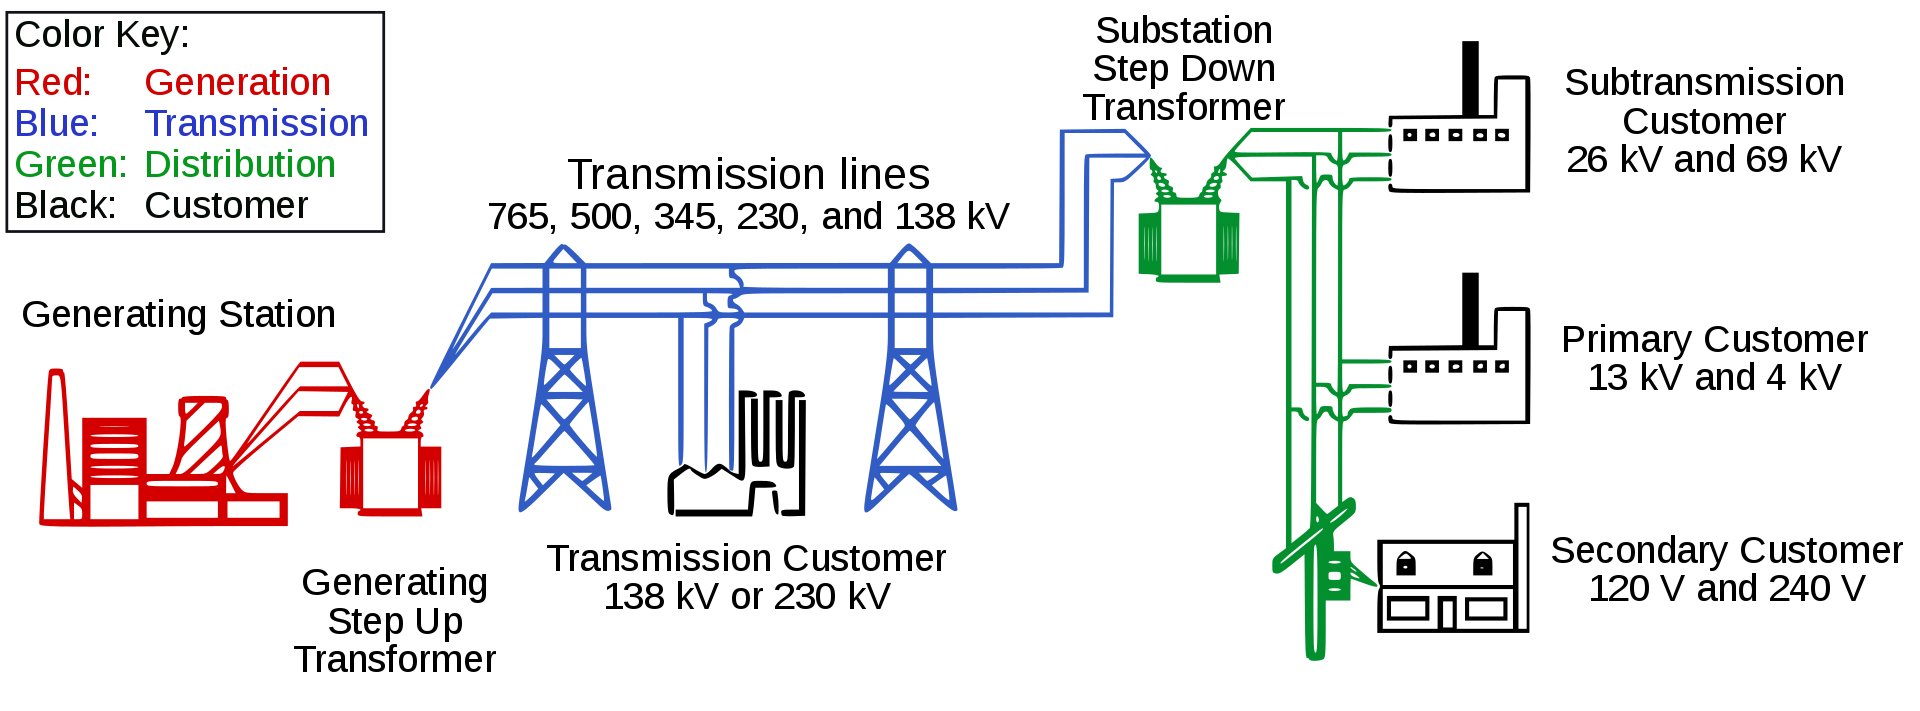
\includegraphics[width=\linewidth]{largeGrid}{\tiny \cite{powersystemSVG} } % image  from https://www.ferc.gov/industries/electric/indus-act/reliability/blackout/ch1-3.pdf
% and https://commons.wikimedia.org/wiki/File:Electricity_grid_simple-_North_America.svg
% 3 Area MiniWECC picture?
Electrical supply connected to demand.\\
%\vspace{1em}
%Power plants connected via transmission lines to cities in different areas. \\
%\vspace{1em}
%A part of `The Grid'.
% picture of north american interconnections
\end{frame}
%------------------------------------------------
\begin{frame}
\frametitle{U.S. Electric Generation}
\begin{center}
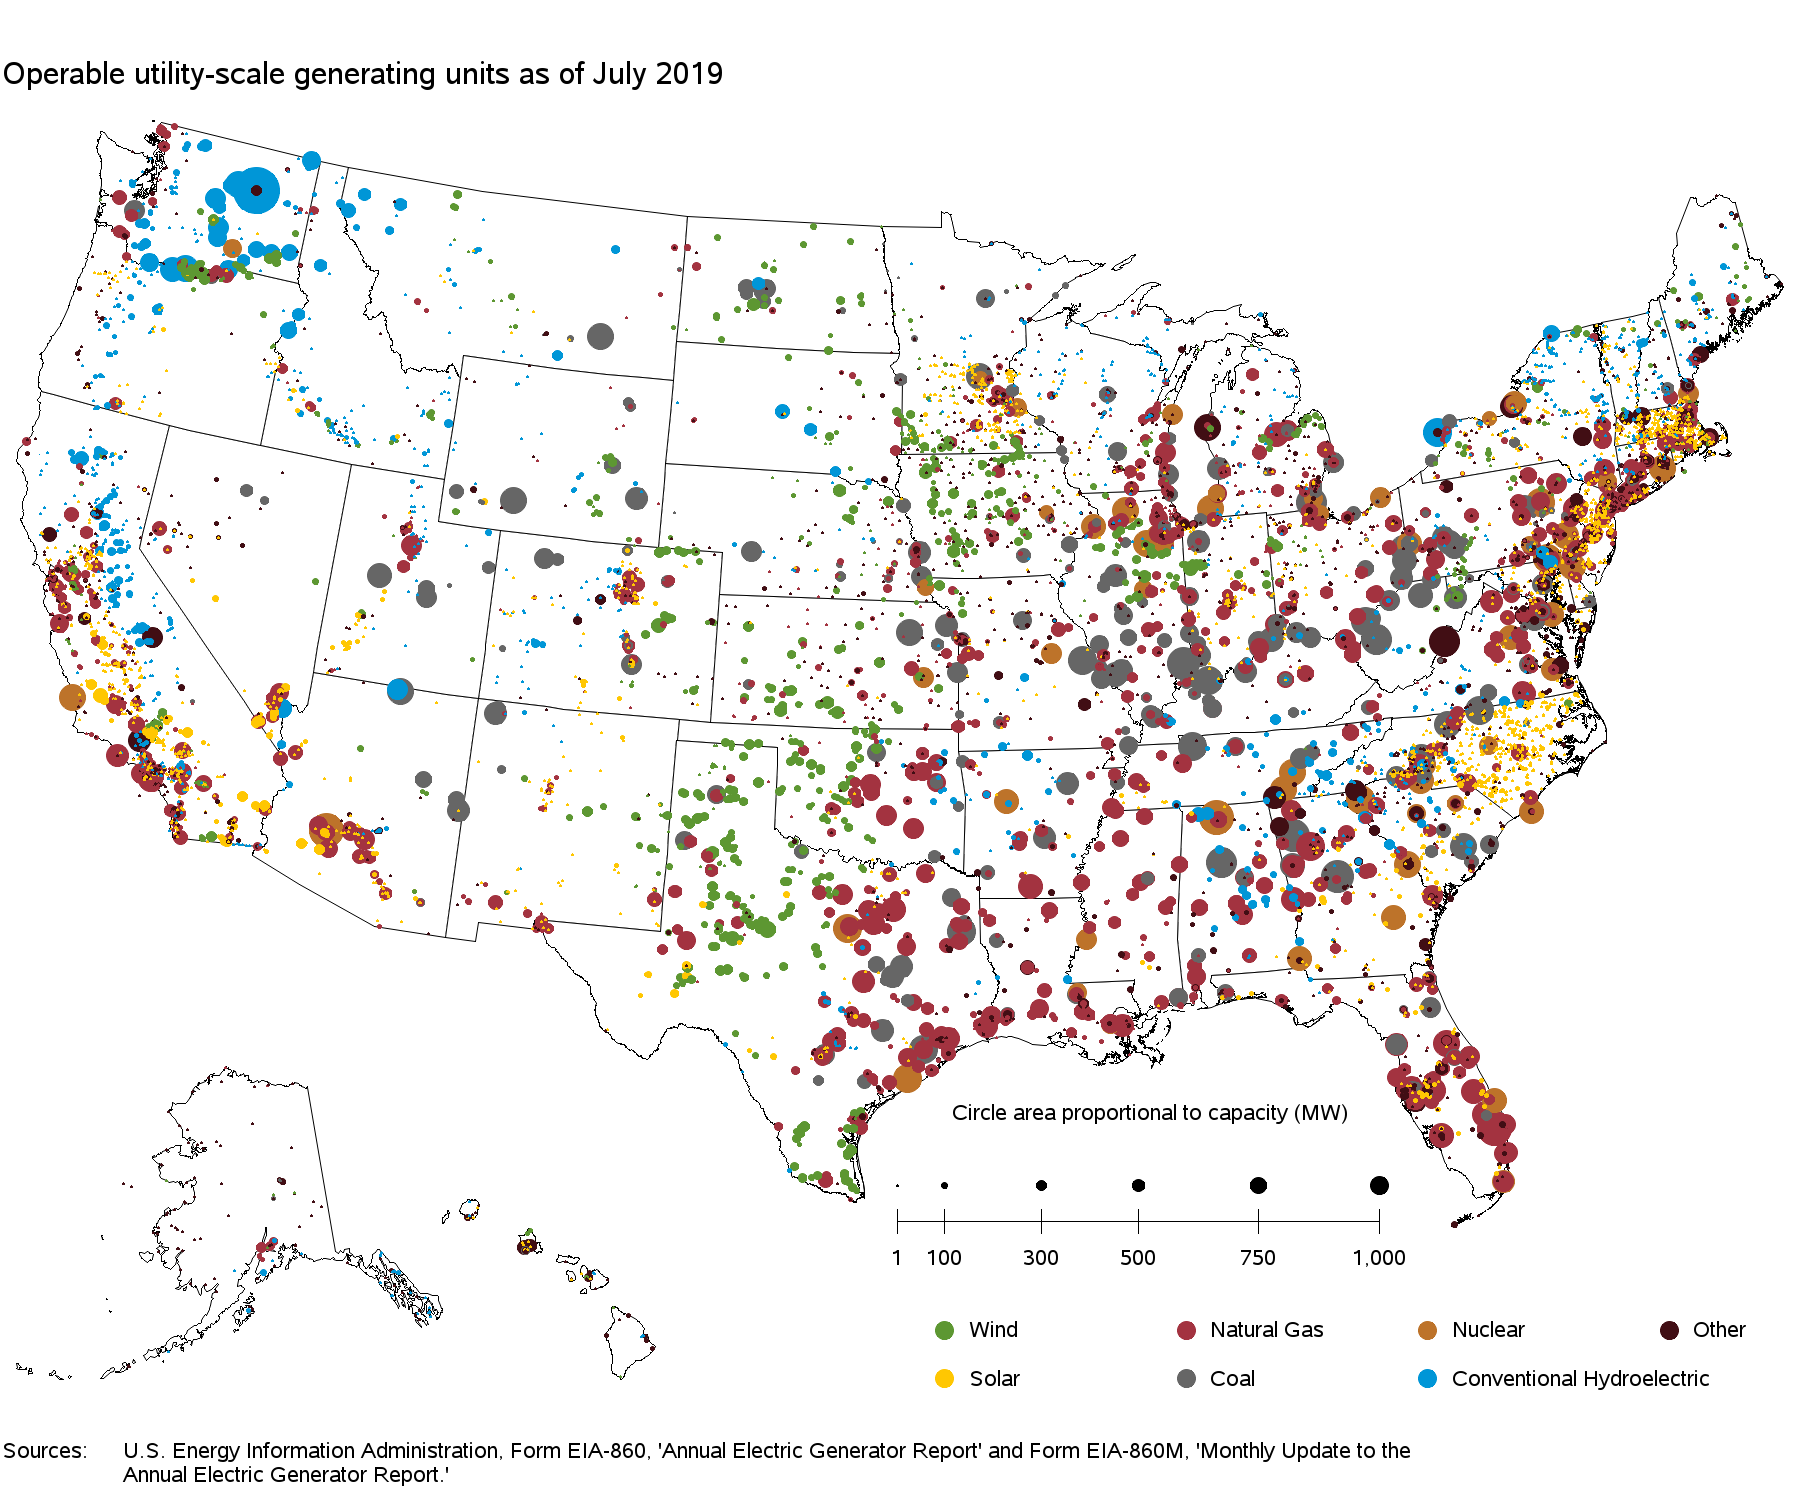
\includegraphics[height=.82\textheight]{july2019map} {\tiny \cite{USgenerationMAP} } % from https://www.eia.gov/electricity/data/eia860m/
\end{center}
\end{frame}
%------------------------------------------------
\begin{frame}
\frametitle{U.S. Electric Transmission Lines}
{\centering%
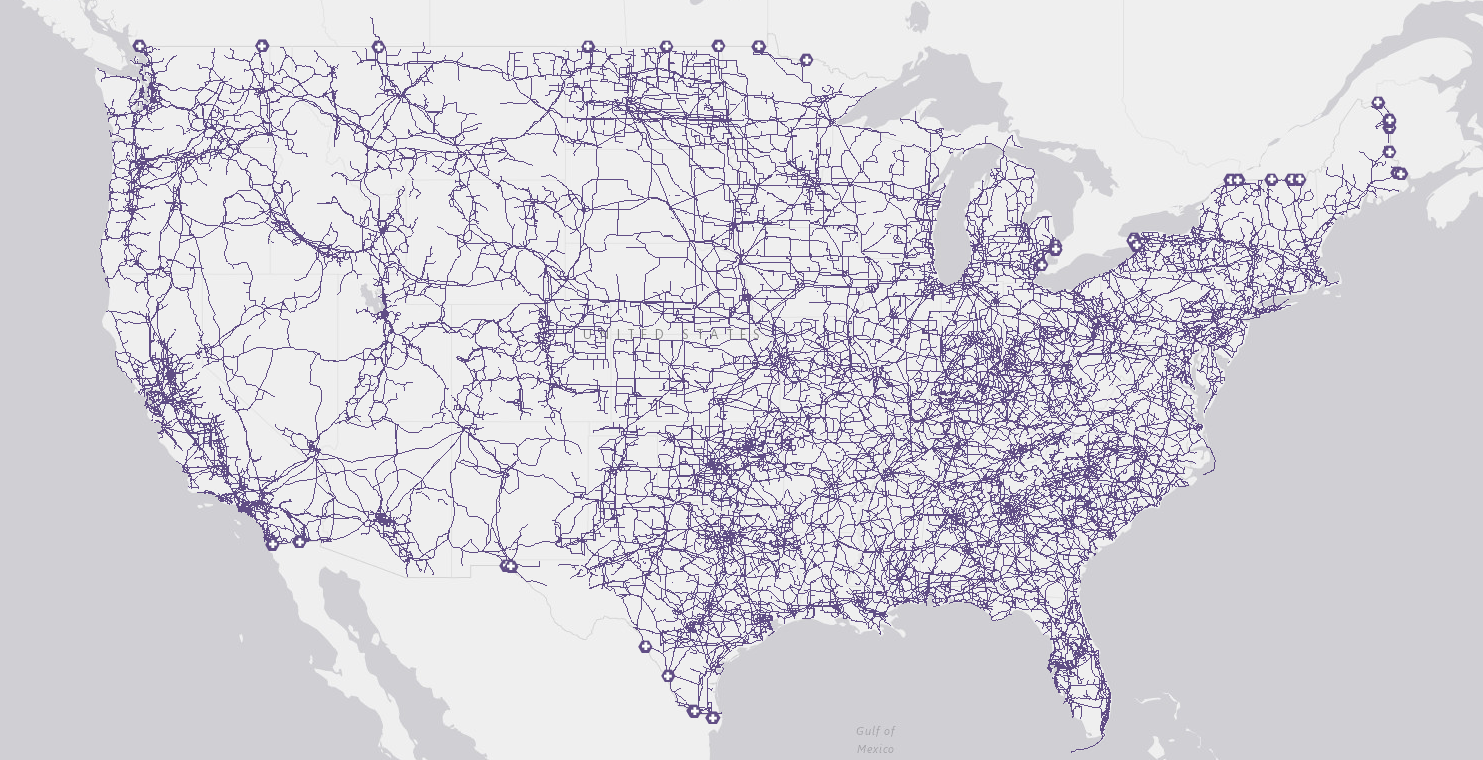
\includegraphics[width=\linewidth]{UStransmission} {\tiny \cite{UStransmissionMAP} } %from https://www.eia.gov/state/maps.php?v=Electricity
}
\end{frame}
%------------------------------------------------
\begin{frame}
\frametitle{Electric Transmission Lines}
{\centering
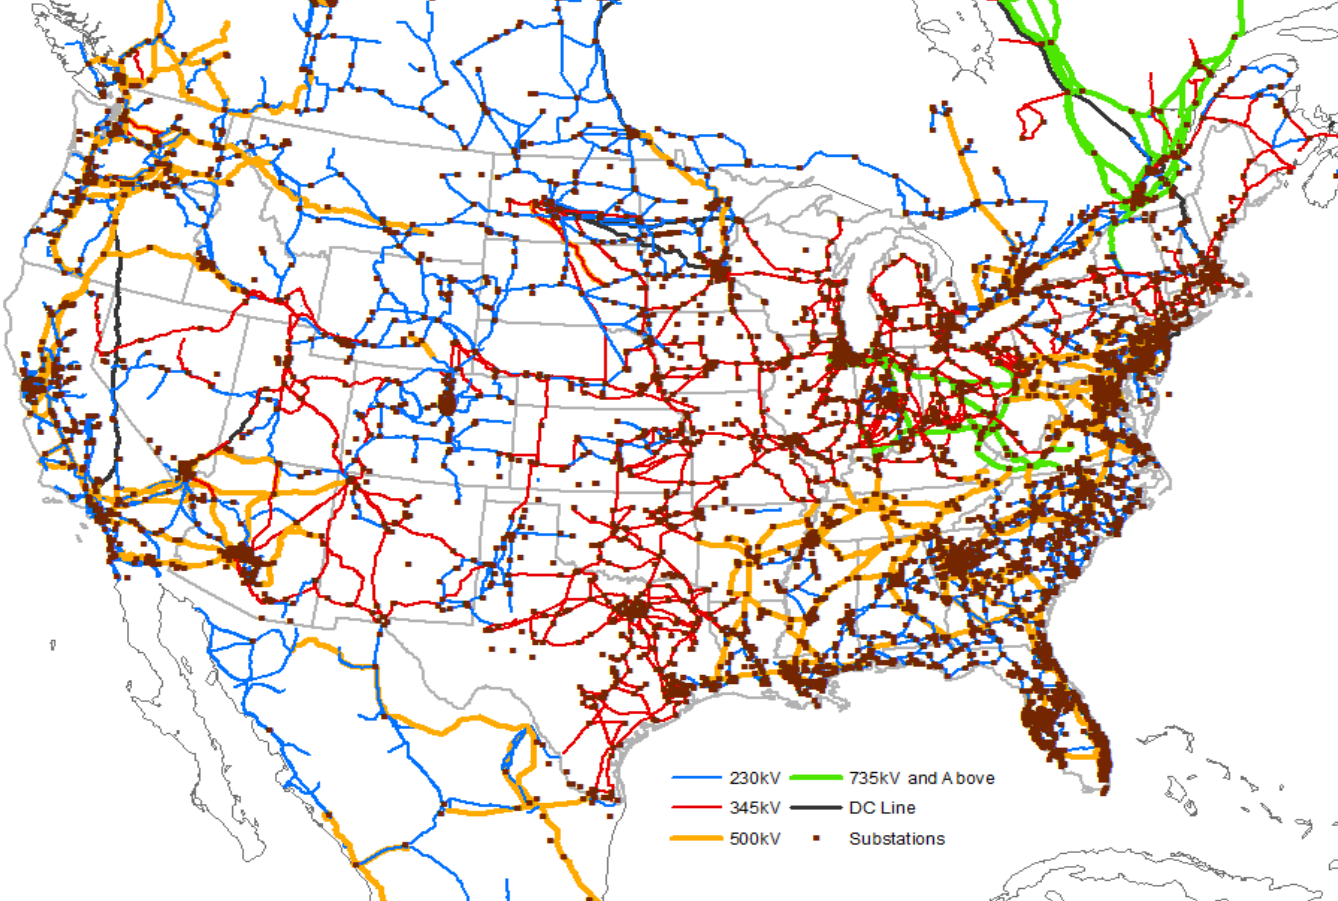
\includegraphics[height=.82\textheight]{xgridPlusSubs} {\tiny \cite{NAtransmissionMAP} }% from Physical Security of the U.S. Power Grid.pdf

}
\end{frame}
%------------------------------------------------
\begin{frame}
\frametitle{Interconnections}
\begin{center}
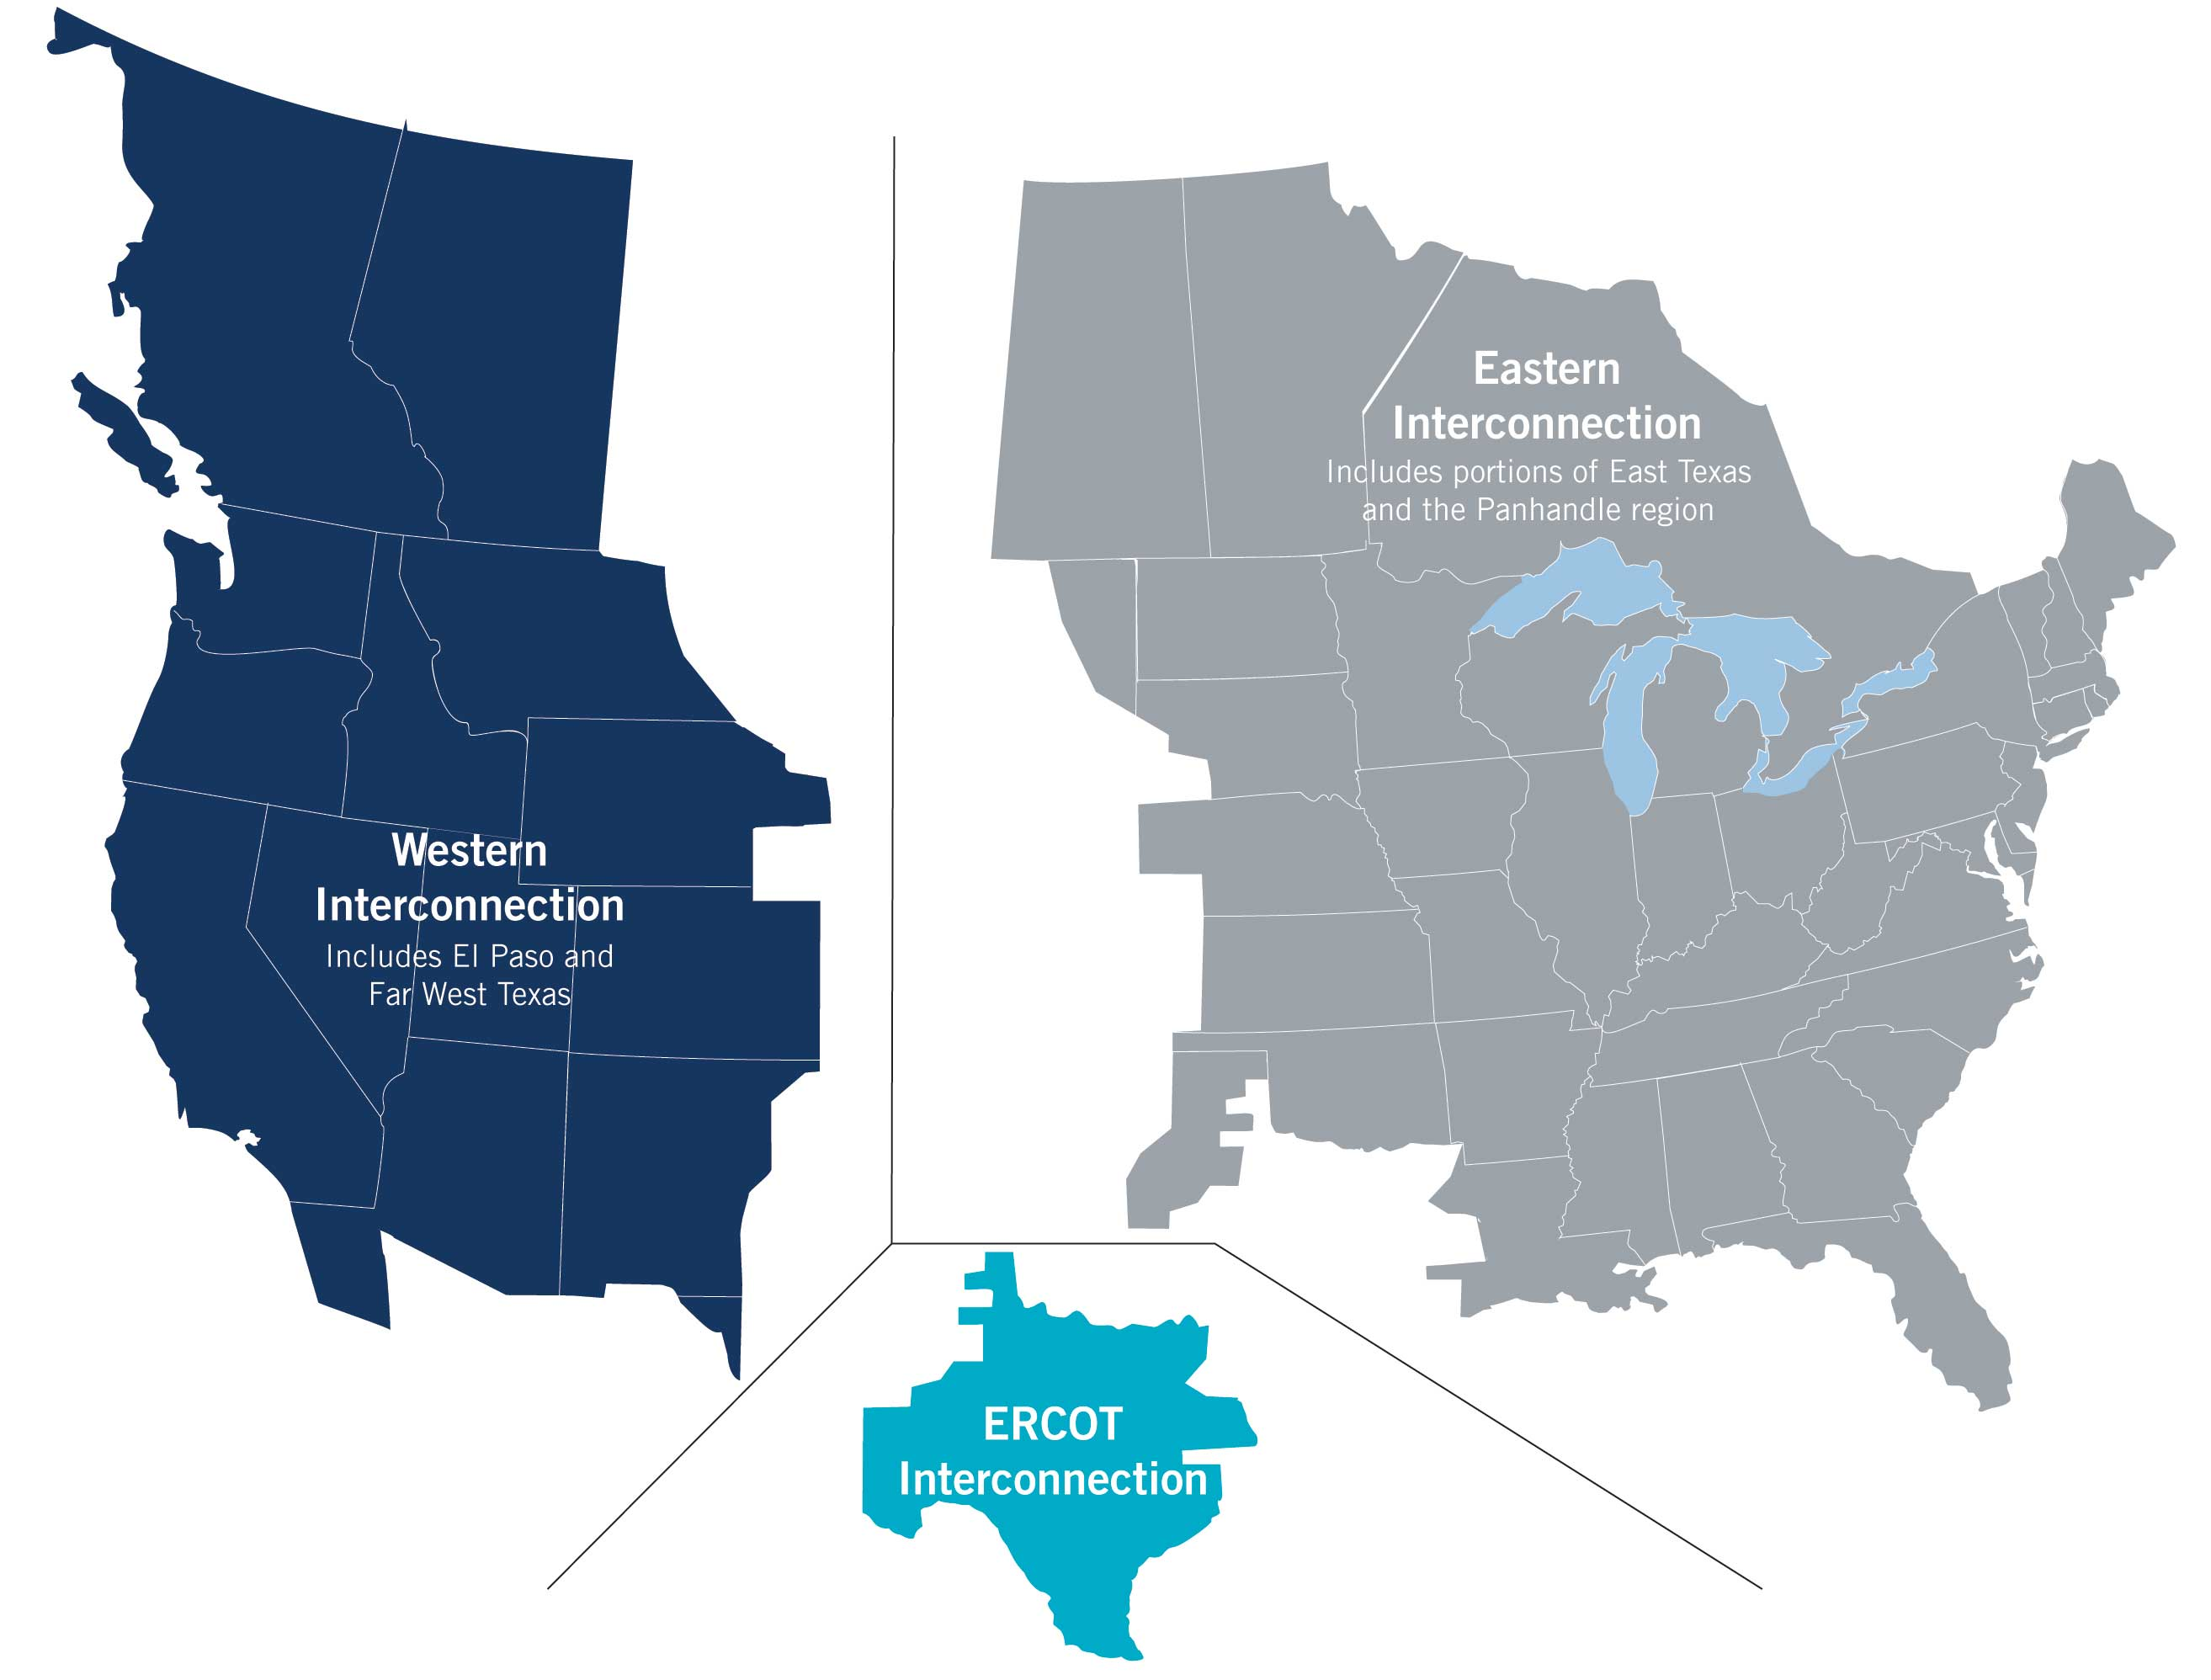
\includegraphics[height=.8\textheight]{InternconnectionBranded}  {\tiny \cite{ercotInterconnections} }% from http://www.ercot.com/news/mediakit/maps
\end{center}

\end{frame}

%------------------------------------------------
\begin{frame}
\frametitle{Industry Software Model}
\framesubtitle{WECC Model}
\begin{columns}
\begin{column}{0.45\textwidth}
   \begin{itemize}
   	\item 4,231 Generators
   	\item 17,210 Lines
 	\item 22 Areas
   	\item 11,048 Loads
	\item 21,879 Buses
\end{itemize}
\end{column}
\begin{column}{0.5\textwidth}
{\tiny \cite{MTlegReport} }
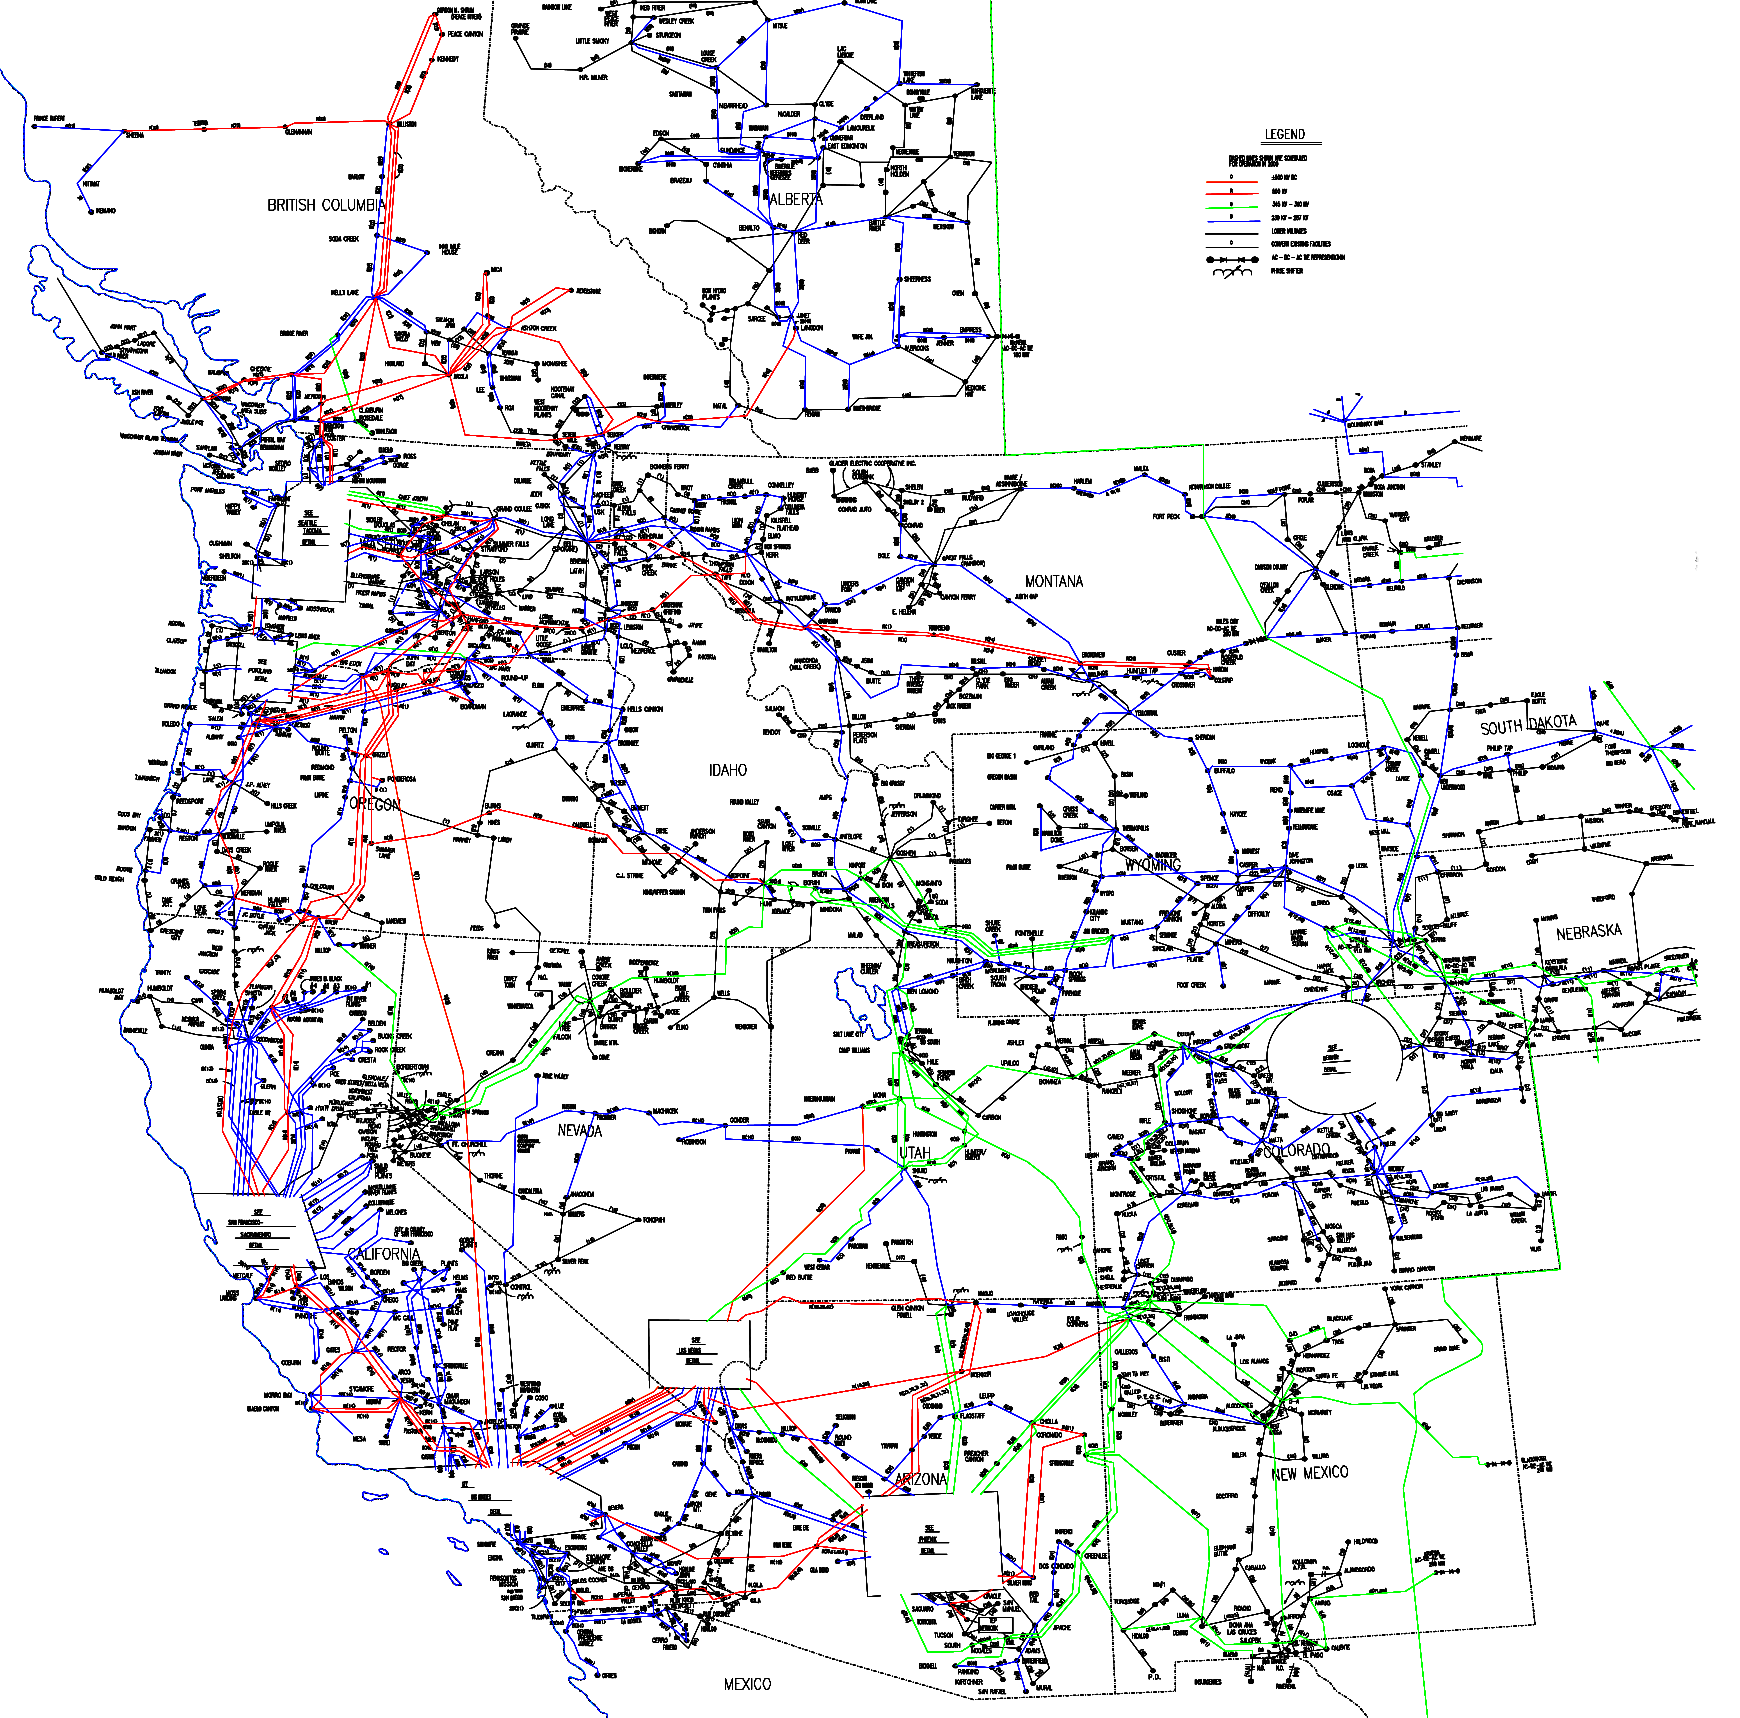
\includegraphics[height=.8\textheight]{WECCauto}  % from Montana electric transmission grid
\end{column}
\end{columns}
\end{frame}

%________________________________________________
\subsection{Operational Structure}
%------------------------------------------------
\begin{frame}
\frametitle{`People in Charge'}
\begin{itemize}
\item \textbf{FERC}{ \footnotesize Federal Energy Regulatory Commission}\\
 Part of the Department of Energy
\item \textbf{NERC}{ \footnotesize
 North American Electric Reliability Corp.}\\
 Aurthority granted by FERC
 \item \textbf{Balancing Authority} (BA) \\
 Manage specific portions of the power system to balance supply and demand and maintain mandatory operating conditions set by FERC and NERC. % abstracted from: https://www.eia.gov/todayinenergy/detail.php?id=27152
\end{itemize}
\end{frame}
%------------------------------------------------
\begin{comment}
\begin{frame}
\frametitle{Six NERC Regions} % how much does this matter?
{\centering
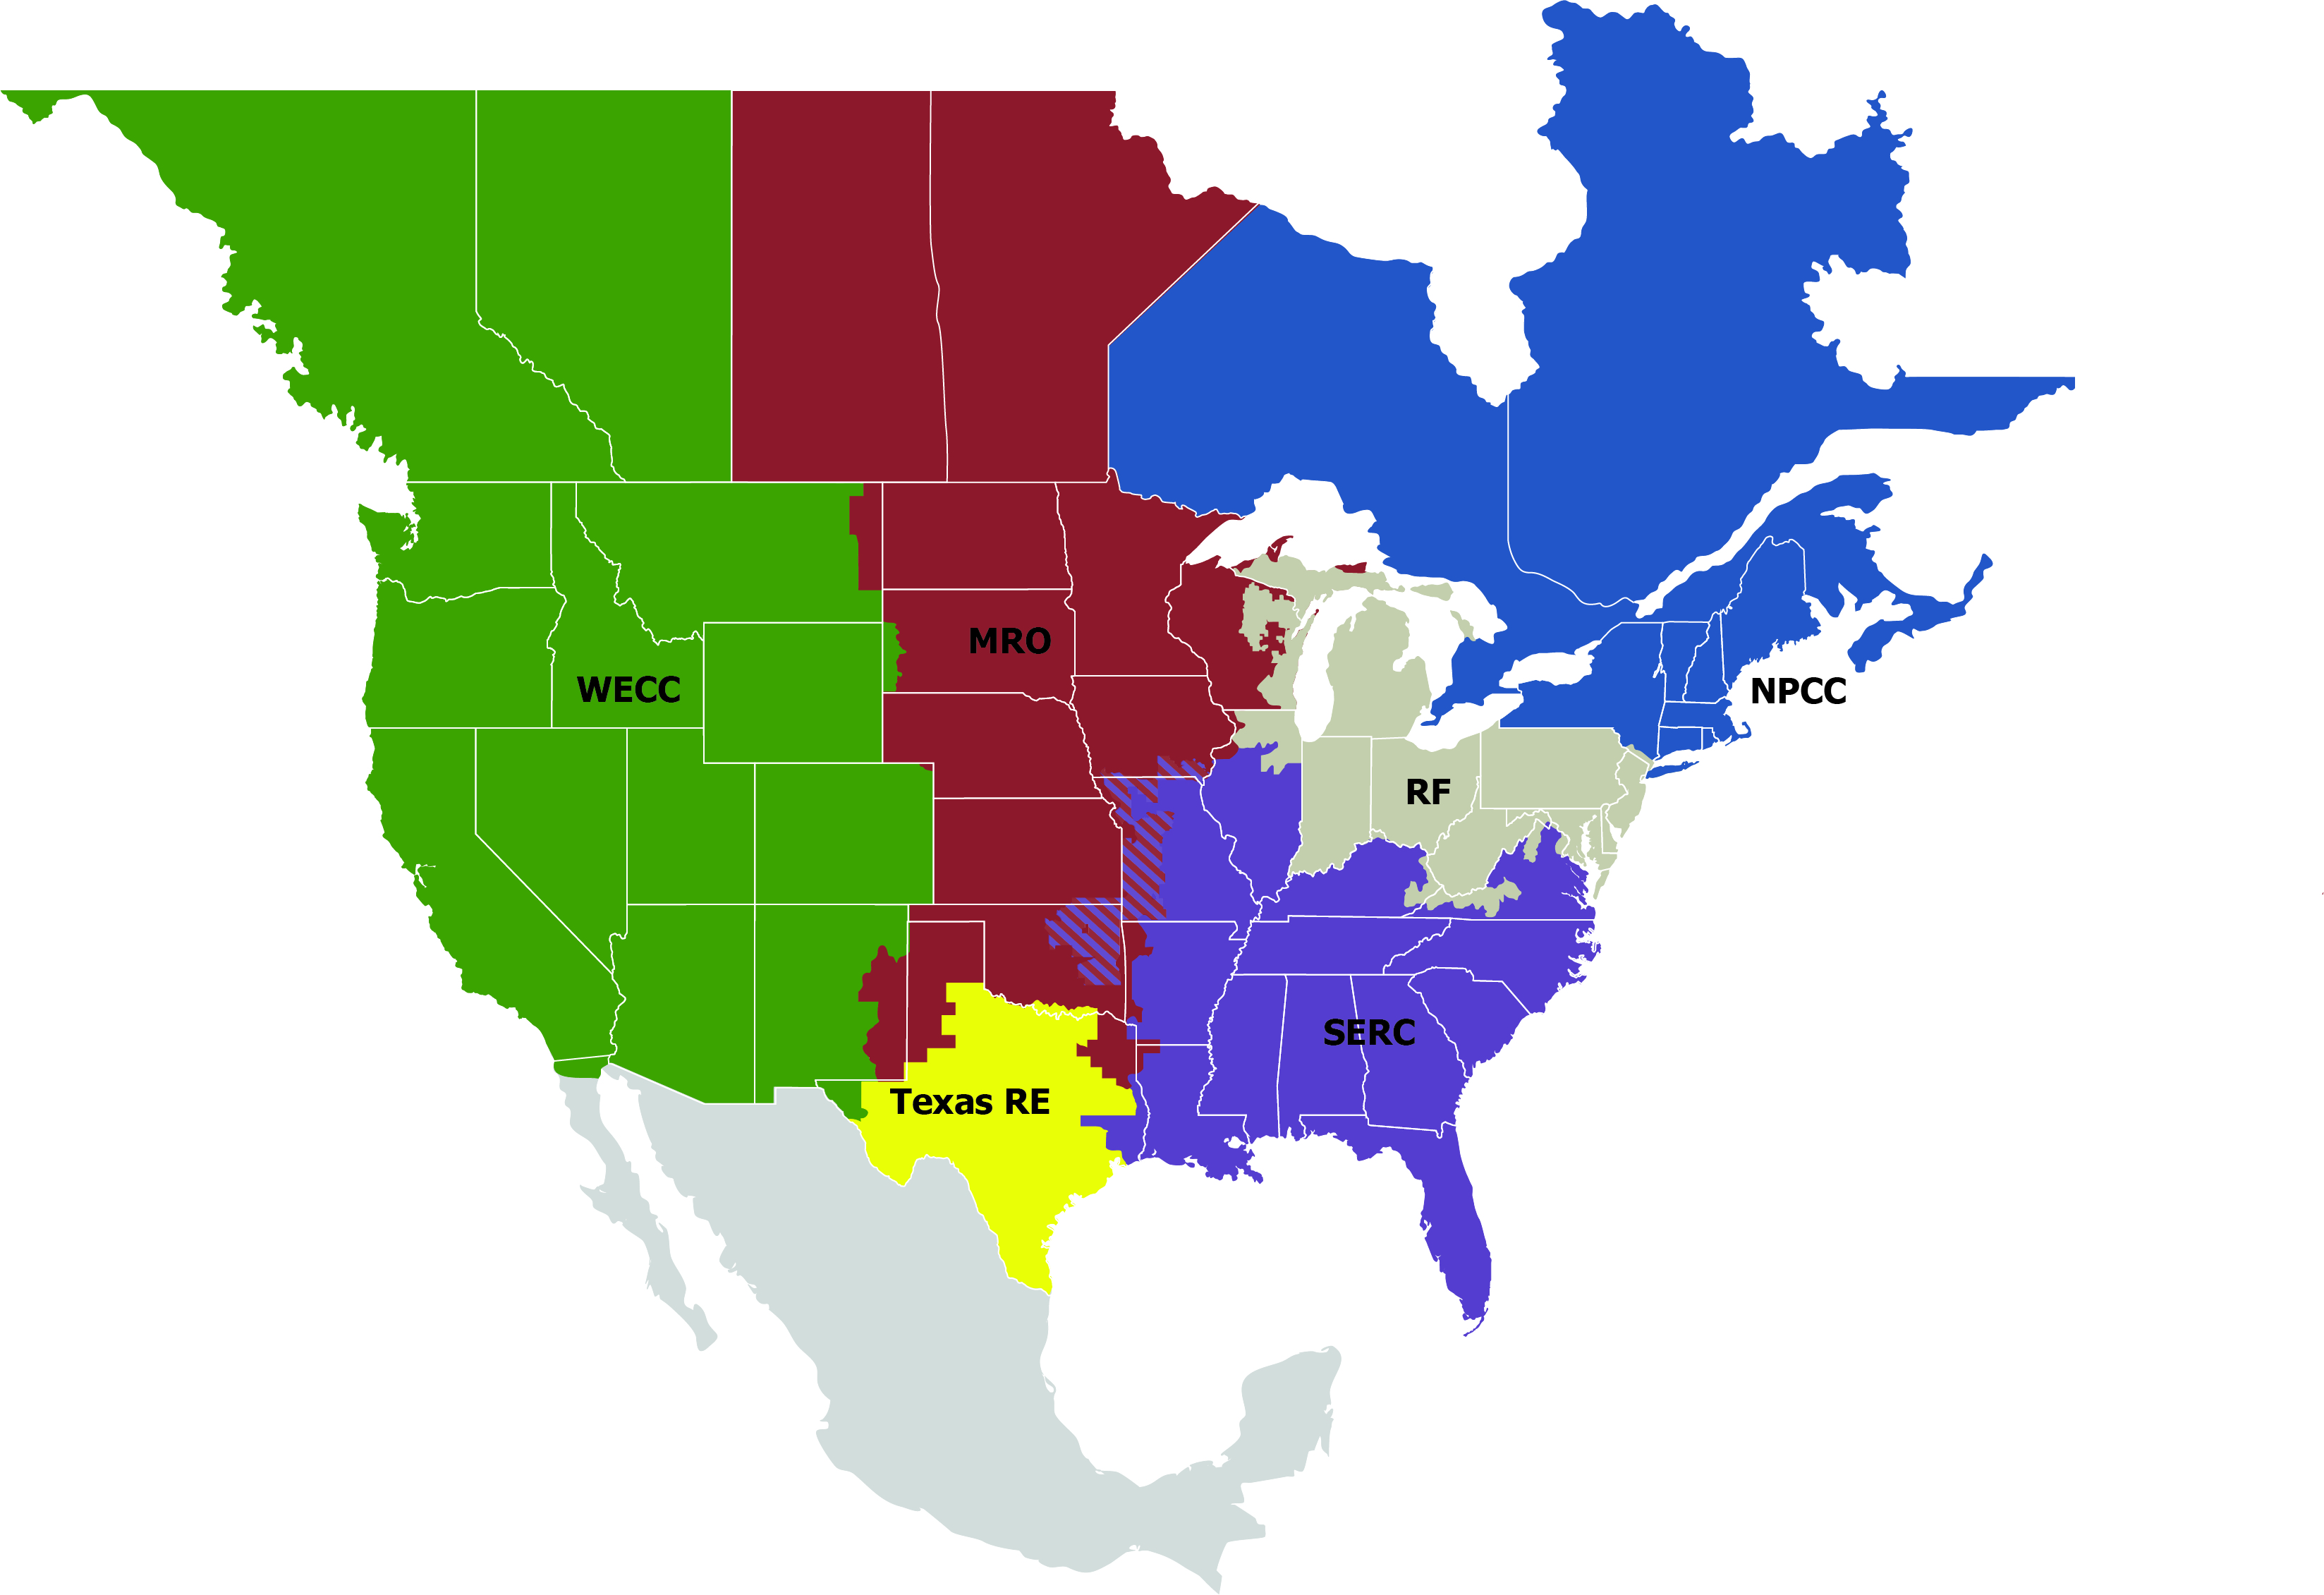
\includegraphics[height=.8\textheight]{NERCregions} % from https://www.nerc.com/AboutNERC/keyplayers/Pages/default.aspx
}
\end{frame}
%------------------------------------------------
\begin{frame}
\frametitle{Main Interconnections} % this may be more of a rehash
{\centering
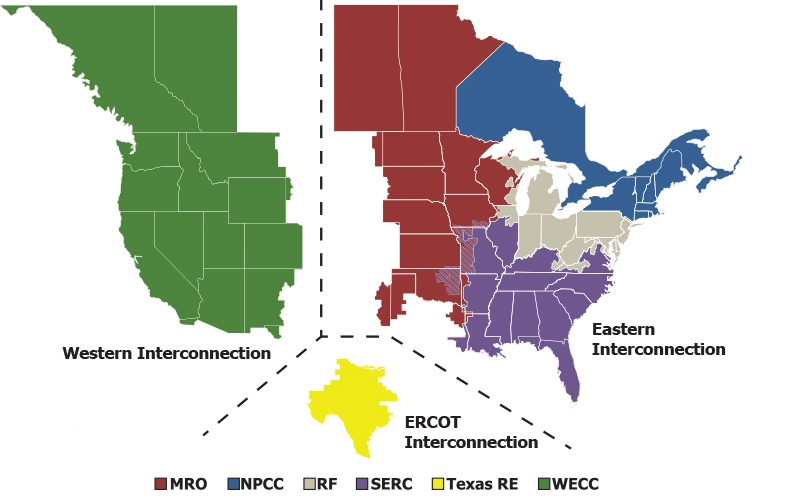
\includegraphics[height=.85\textheight]{NERCInterconnectionsEDIT} % edited from https://www.nerc.com/AboutNERC/keyplayers/Pages/default.aspx
}
\end{frame}
\end{comment}
%------------------------------------------------
\begin{frame}
\frametitle{Balancing Authorities (BAs)}\ \vspace{.5em}
% Roughtly 60, circles indicitive of size
\begin{center}
\vspace{-1.5em}
\href{https://www.eia.gov/realtime_grid/}%
{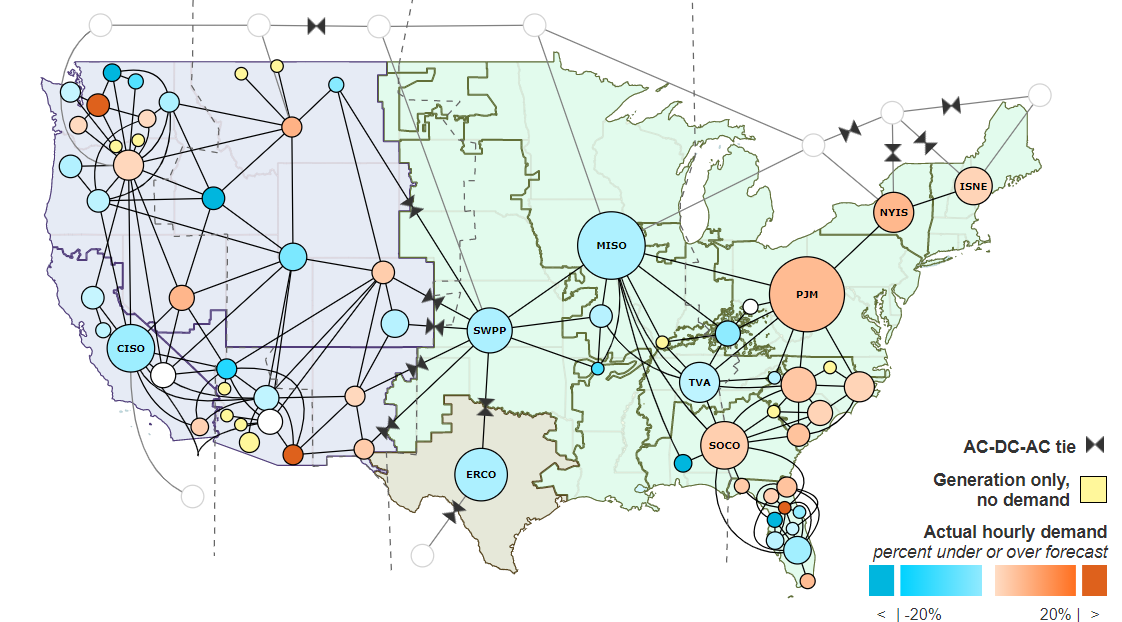
\includegraphics[width=.95\linewidth]{BAs}} % from https://www.eia.gov/realtime_grid/
\end{center}
\vspace{-1em}
{\tiny \cite{BAinformation} }
\end{frame}
%------------------------------------------------
\begin{frame}
\frametitle{BA Action - Forcasting} %\ \vspace{.5em}
\begin{center}
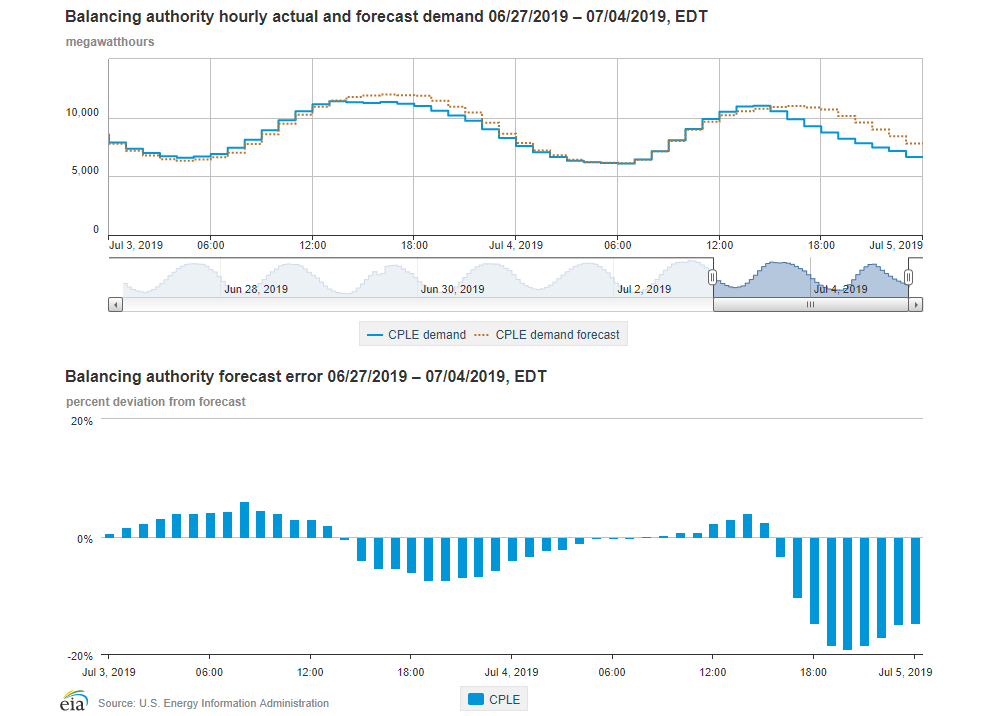
\includegraphics[height=.82\textheight]{BAforcast} {\tiny \cite{BAinformation} }% https://www.eia.gov/realtime_grid/#/data/graphs?end=20190704T18&start=20190627T18&bas=000001&regions=0&errSeriesType=S
\end{center}

\end{frame}
%------------------------------------------------
\begin{frame}
\frametitle{BA Action - Interchange} %\ \vspace{.5em}
\begin{center}
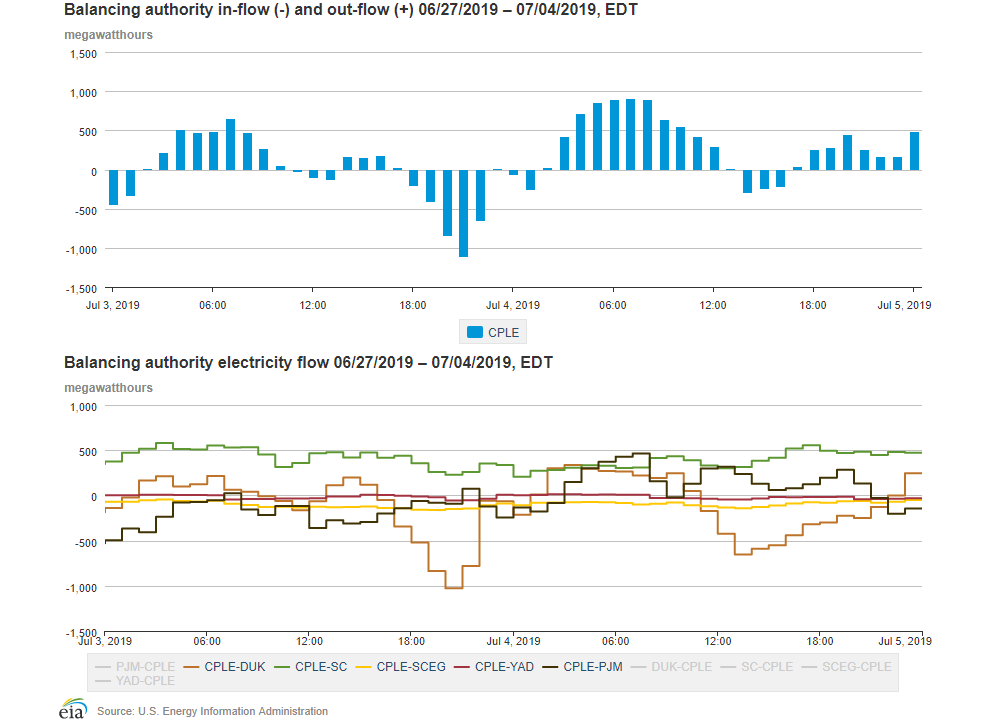
\includegraphics[height=.82\textheight]{BAinterchange} {\tiny \cite{BAinformation} }% https://www.eia.gov/realtime_grid/#/data/graphs?end=20190704T18&start=20190627T18&bas=000001&regions=0&errSeriesType=S
\end{center}

\end{frame}
%------------------------------------------------
\begin{frame}
\frametitle{BA Action - Interchange Error} \ \vspace{.5em}
$\approx$ Area Control Error
{\centering
{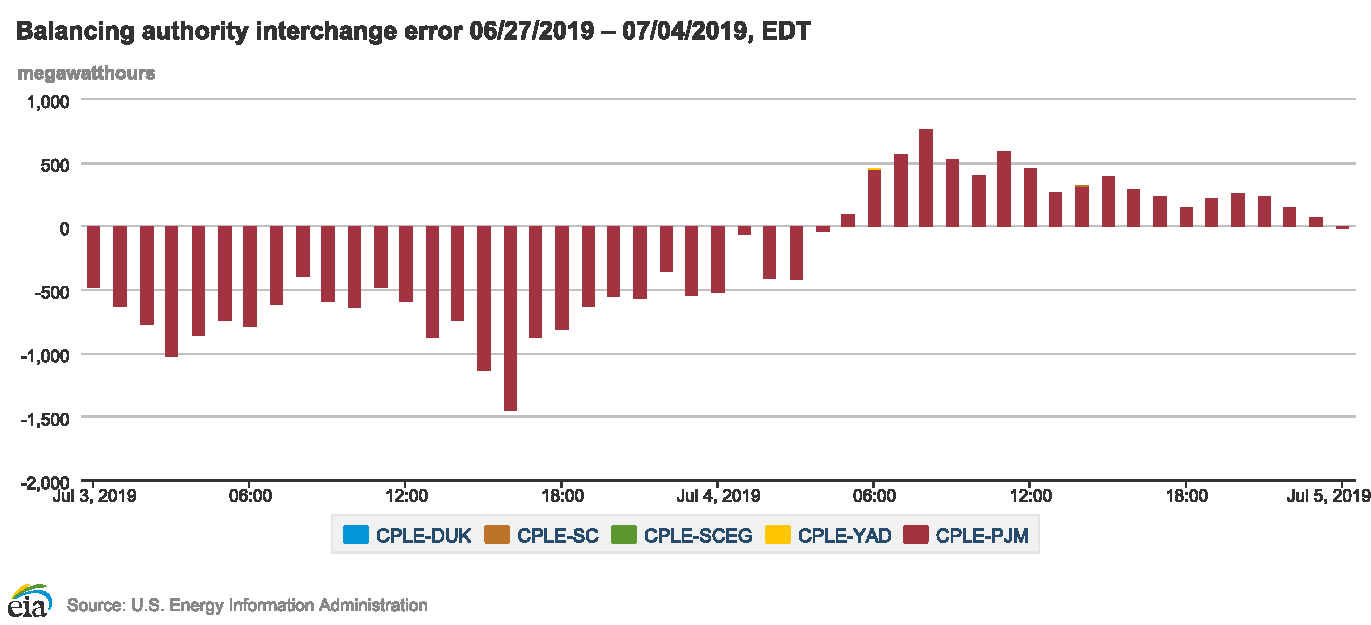
\includegraphics[height=.6\textheight]{chart4}} {\tiny \cite{BAinformation} }% https://www.eia.gov/realtime_grid/#/data/graphs?end=20190704T18&start=20190627T18&bas=000001&regions=0&errSeriesType=S
}

\end{frame}
%------------------------------------------------

%************************************************
\section{Long-Term Dynamics}
%________________________________________________
\subsection{Explanation of Wording}
%------------------------------------------------
\begin{frame}
\frametitle{What is Long-Term?}
%Long-term describes the amount of time required for events of interest to occur and the simulation length to be executed.
\begin{columns}
	\begin{column}{0.7\textwidth}
		\begin{center}
			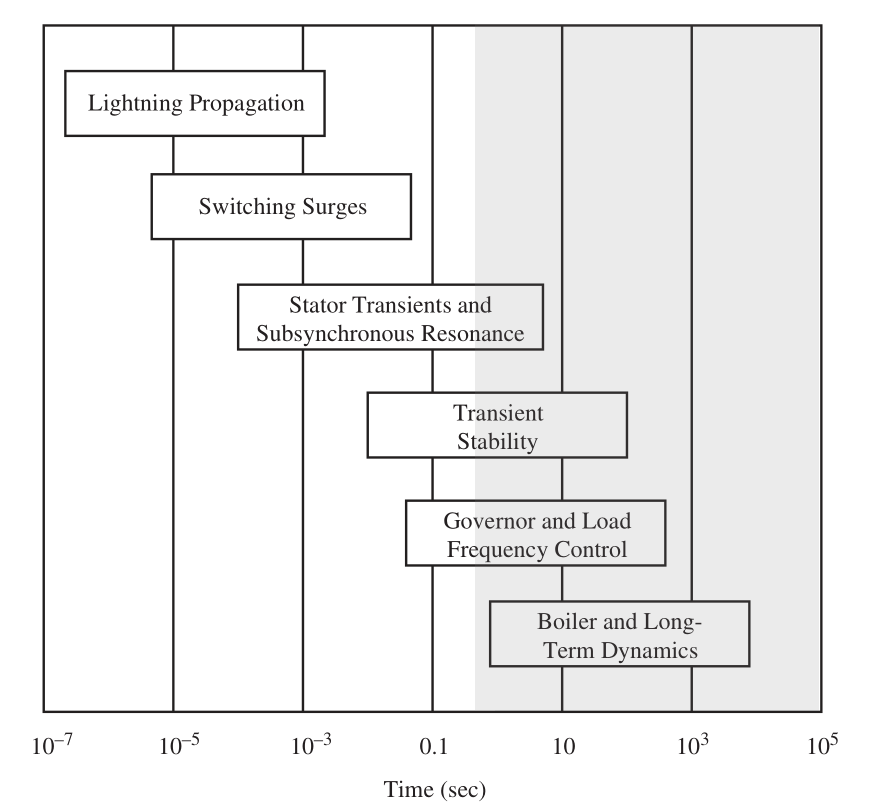
\includegraphics[height=.8\textheight]{timeScalesHL}{\tiny\cite{SauerPaiChow}} 
		\end{center}
	\end{column}
	\begin{column}{0.5\textwidth}
	   \begin{itemize}
			\small
			\item 1 sec $\leftrightarrow$ hours \\
			$\therefore$ 
			\item 10$\rightarrow$60 minute simulations
			\item 1 sec time step
	\end{itemize}
	\end{column}

\end{columns}
\end{frame}
%------------------------------------------------
\begin{frame}
\frametitle{What is Dynamic Simulation?}
A computer's mathematical solution to how a system may change over time.\\% in response to certain inputs and known starting conditions.\\ % Simulation of system changing over time
\vspace{1em}
Think solving ODE's.\\
\vspace{1em}
How certain qualities of a power system may change over time in response to a known perturbance.
\end{frame}
%------------------------------------------------
\subsection{Dynamic Concepts of Interest}
%------------------------------------------------
\begin{frame}
\frametitle{Frequency ($\omega$)}
%Direct link - electric demand always met. If there isn't enough generation, the kinetic energy stored as a moving inertia in a generator is converted to electric energy and the generator slows down.
\begin{minipage}[t][.55\textheight][t]{\textwidth}
%\begin{columns}
%\begin{column}{0.4\textwidth}
	\begin{minipage}{.4\linewidth}
\vspace{-2em}
\[ \dot{\omega}_{sys} = \dfrac{P_{acc, sys}}{2H_{sys}\omega_{sys}(t) } \]
\[ P_{acc} = P_{gen} - P_{load} \]
	
\end{minipage}%
%\end{column}
%\begin{column}{0.6\textwidth}
\begin{minipage}{.6\linewidth}
\vspace{-2em}
    \begin{center}
     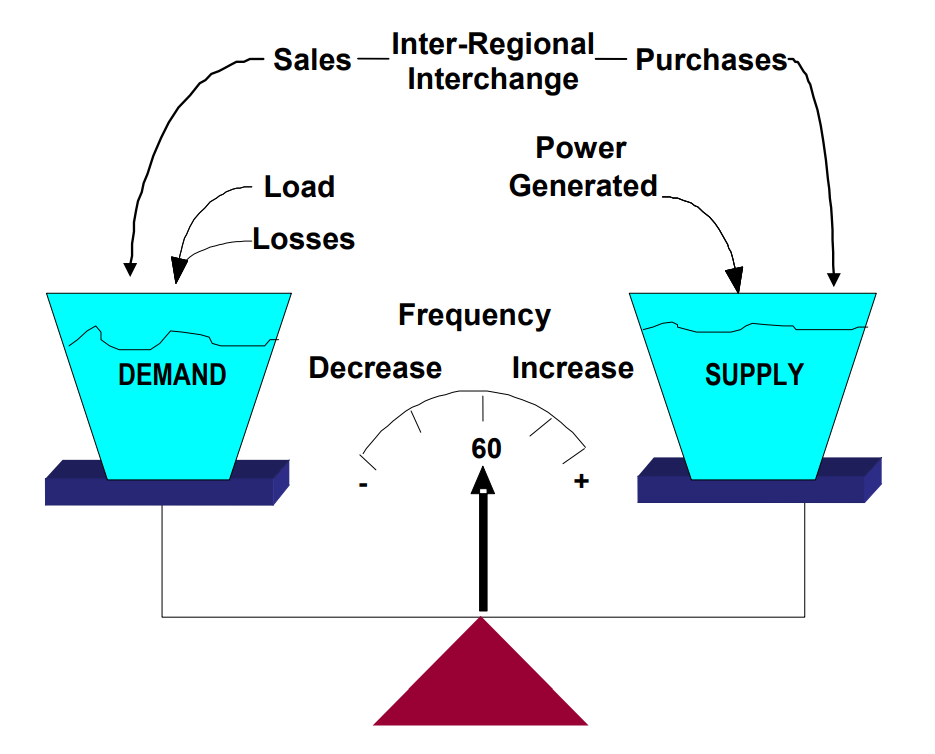
\includegraphics[width=\linewidth]{freqScale}   {\tiny\cite{freqScale}}%  from comm-OC-RS_Related_Resources-nerc balancing and frequency control 040520111.pdf
     \end{center}
\end{minipage}
%\end{column}
%\end{columns}
\end{minipage}
Electric load always met.\\
\vspace{.5 em}
Load and losses always changing.
\end{frame}
%------------------------------------------------
\begin{frame}
\frametitle{Automatic Controls}
\begin{center}
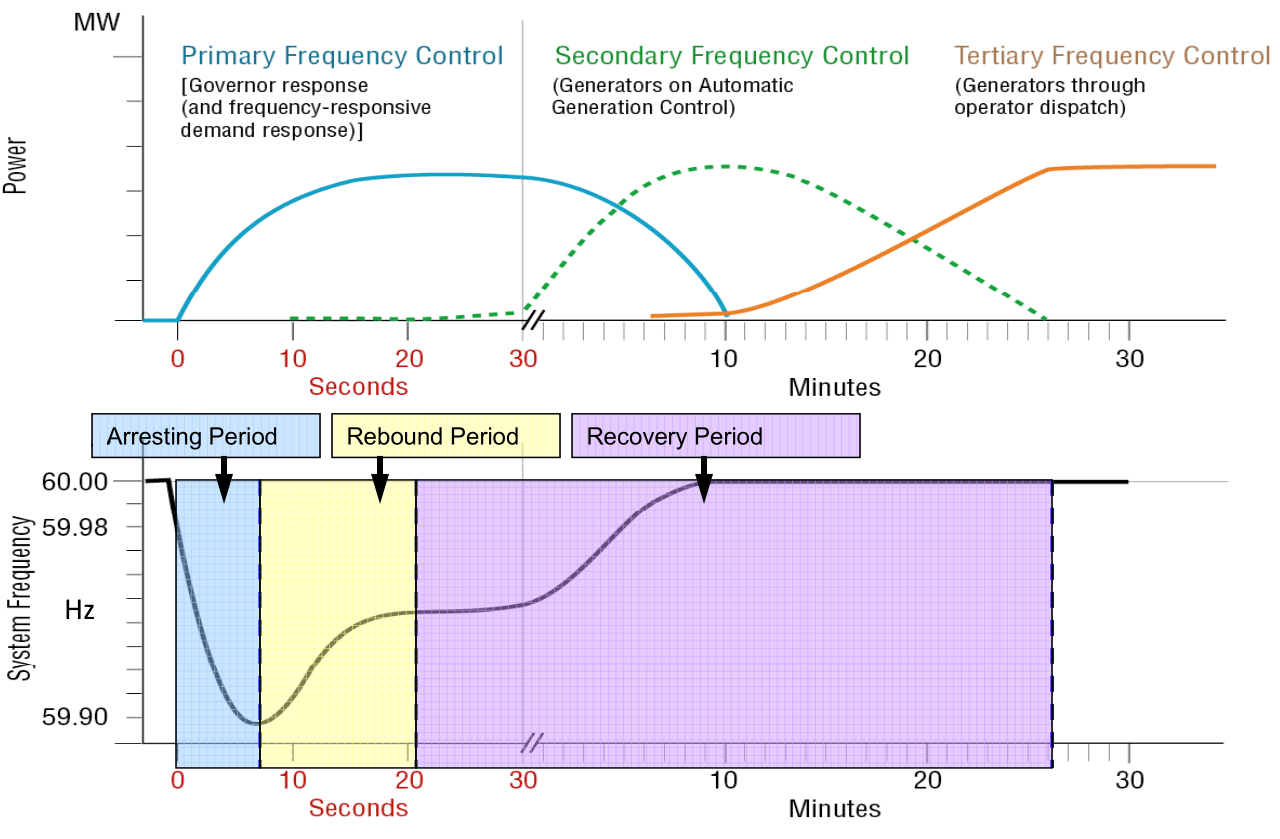
\includegraphics[height=.82\textheight]{ctrlReactionFlip} {\tiny\cite{ctrlTimeScale}}% modified from Generator Governor and Information Settings Webinar NERC
\end{center}
\end{frame}
%------------------------------------------------
\begin{frame}
\frametitle{Turbine Speed Governors}
\framesubtitle{Primary Control}

Purpose: Adjust turbine mechanical power to arrest frequency decline.\\
\vspace{.5em}

Dynamic Variable: Fuel Valve Position 
% model of tgov1?
{\centering\includegraphics[width=\linewidth]{../../ResearchDocs/TEX/models/tgov1/tgov1}}

\end{frame}
%------------------------------------------------
\begin{frame}
\frametitle{Automatic Generation Control}
\framesubtitle{Secondary Control}

Purpose: Eliminate Area Control Error\\
\vspace{.5em}
Dynamic Variable: Area Control Error
%(AGC), also knows as Load Frequency Control or LFC)
%\\
%Adjusts generator nominal operating set point to remove any inadvertent interchange and restore system frequency to 60 Hz. Classified Secondary Control.
% kundur pic... p378 firug 9.1
\begin{center}
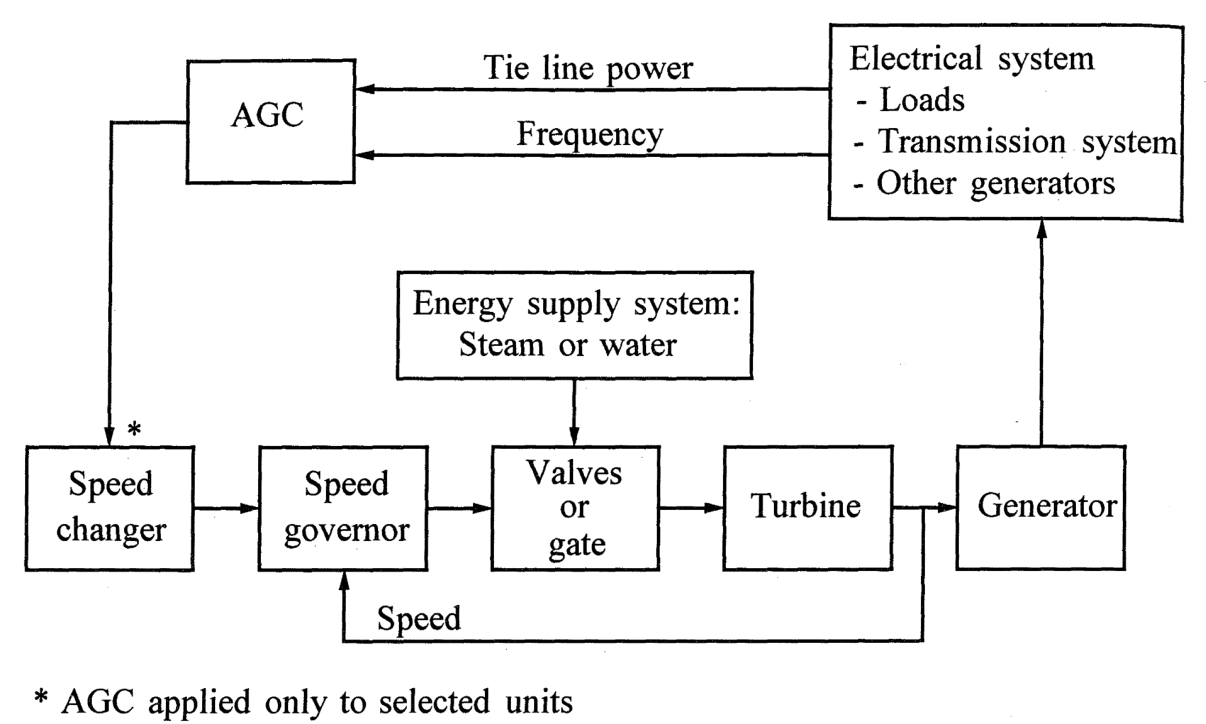
\includegraphics[height=.55\textheight]{AGCblockdiagram}
{\tiny\cite{Kundur}}
\end{center}
\end{frame}
%------------------------------------------------


%************************************************
\section{Time-Sequenced Power Flows}
%________________________________________________
\subsection{Explanation of Computational Approach}
%------------------------------------------------
\begin{frame}
\frametitle{What is a Power Flow?}
%\begin{columns}
%	\begin{column}{.5\linewidth}
		A steady state power system solution.\\% to all bus voltages, bus voltage angles, and real  and reactive power of a system.\\
		% A sonlution to a system of non-linear equations solved by iteration.
		%\vspace{1em}
		A \emph{snapshot} of a stable power system. \\% not dynamic
		
%	\end{column}
%	\begin{column}{.5\linewidth}

\begin{center}
	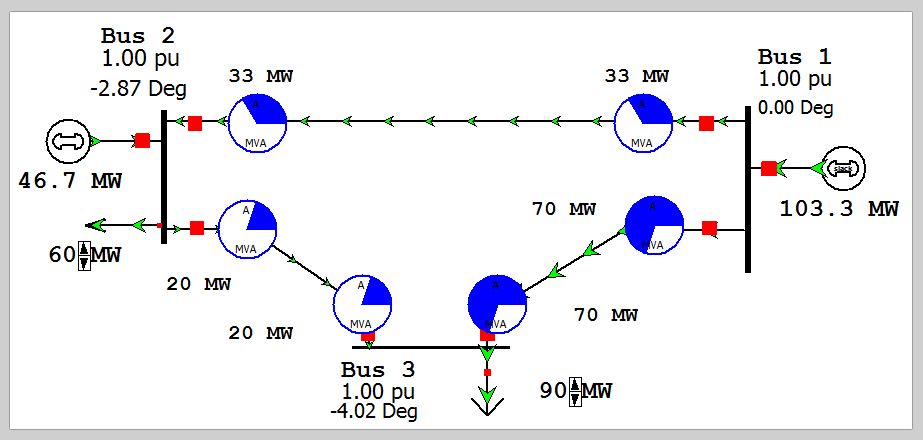
\includegraphics[width=.6\linewidth]{powerFlowSingle} 
\end{center}

	
		Power flows are not dynamic.
%	\end{column}
%\end{columns}

\end{frame}
%------------------------------------------------
\begin{frame}
\frametitle{Time-Sequenced Power Flows?}
Power flows arranged in sequence to give the illusion of time.\\
%\vspace{1em}
%A \emph{flip book} of \emph{snapshots}.\\
\begin{center}
	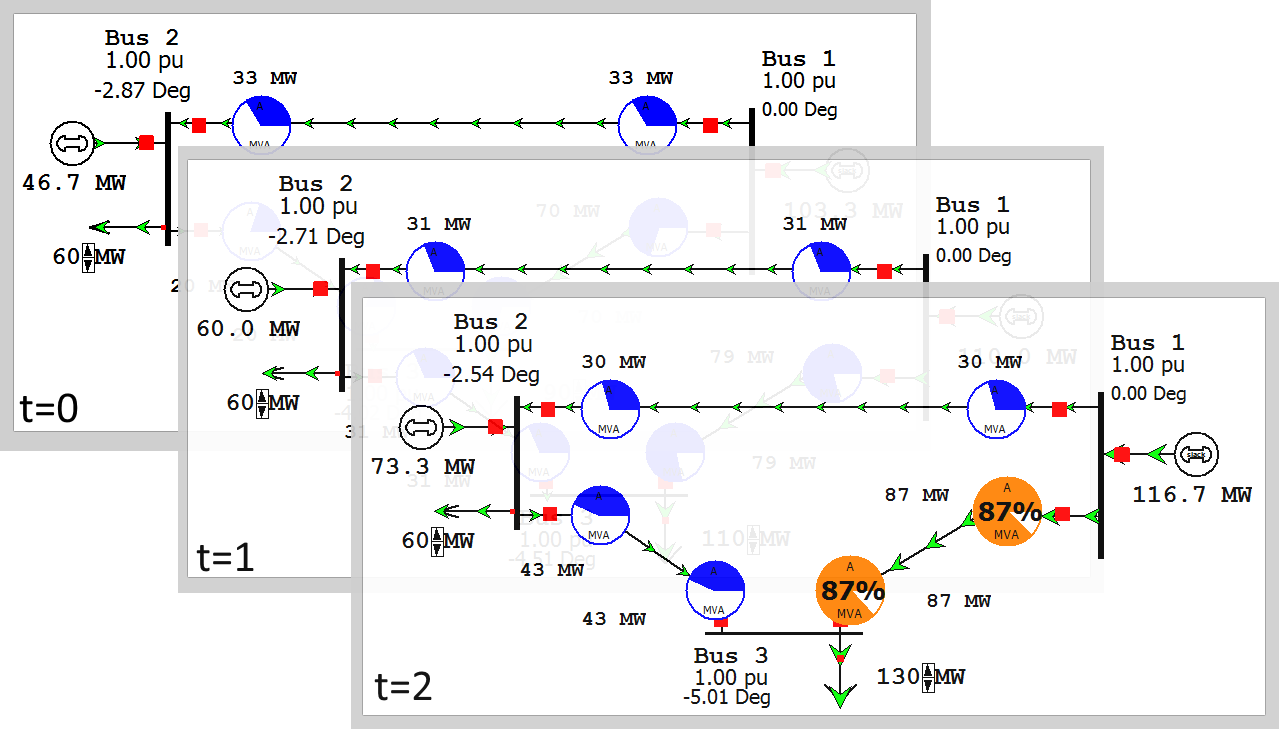
\includegraphics[width=.8\linewidth]{powerFlowSequence}
\end{center}
%\vspace{1em}
%Dynamics calculated between power flows.%\\(i.e frequency, valve position, etc. )\\
\end{frame}
%________________________________________________
\subsection{Rational for Computational Approach}
%------------------------------------------------
\begin{frame}
\frametitle{Why use this method?}
Allows for:
\begin{itemize}
\item Simplifications
\item Greater access to data
\item Customizable models
\item Modern programming language
\item Further future work
\end{itemize}
\end{frame}
%************************************************
\section{Recap}
%________________________________________________
\subsection{General Project Overview}
\begin{frame}
\frametitle{So, what's happening?}
Essentially:
\begin{itemize}
	\item Executing computer simulations of the western interconnection that are  over 10 minutes long.
	\item Simulation `time steps' are a sequence of power flows (\emph{snapshots})
	\item Additional dynamic calculations are performed between each `time step'.
\end{itemize}

\end{frame}
%------------------------------------------------
\begin{frame}
\frametitle{And why?}
To study engineering problems involving:
\begin{itemize}
	\item Long-term events (i.e. Wind Ramps)
	\item Multi-Area Power Interactions
	\begin{itemize}
		\item Governor and AGC interaction
		\item Governor and AGC settings		
	\end{itemize}
	\item Ways to reduce machine effort while meeting reliability standards.
\end{itemize}
\end{frame}
%************************************************
\section{Quick Results}
%________________________________________________
\subsection{Quick Validation}
%------------------------------------------------
\begin{frame}
\frametitle{Software Model}
\framesubtitle{miniWECC}
\begin{columns}
	\begin{column}{0.45\textwidth}
		\begin{itemize}
			\item 34 Generators
			\item 104 Lines
			\item 3 Areas
			\item 23 Loads
			\item 120 Buses
		\end{itemize}
	\end{column}
	\begin{column}{.5\textwidth}
		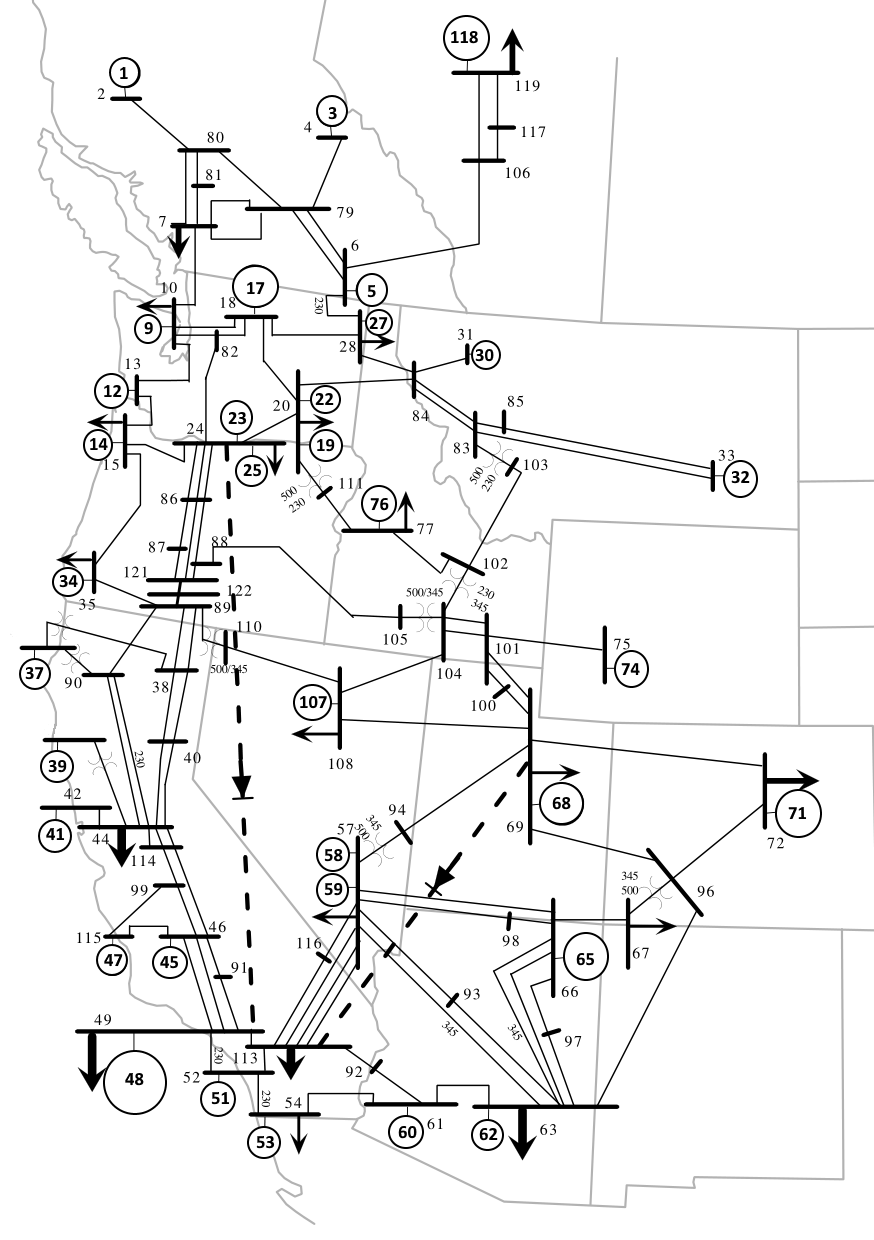
\includegraphics[height=.8\textheight]{miniWECCpres} 
		{\tiny\cite{RJminiWECC}}% from RJ paper...
	\end{column}
\end{columns}
\end{frame}
%------------------------------------------------
\begin{frame}
\frametitle{Plot Explanation}\ \\
\vspace{.25em}
		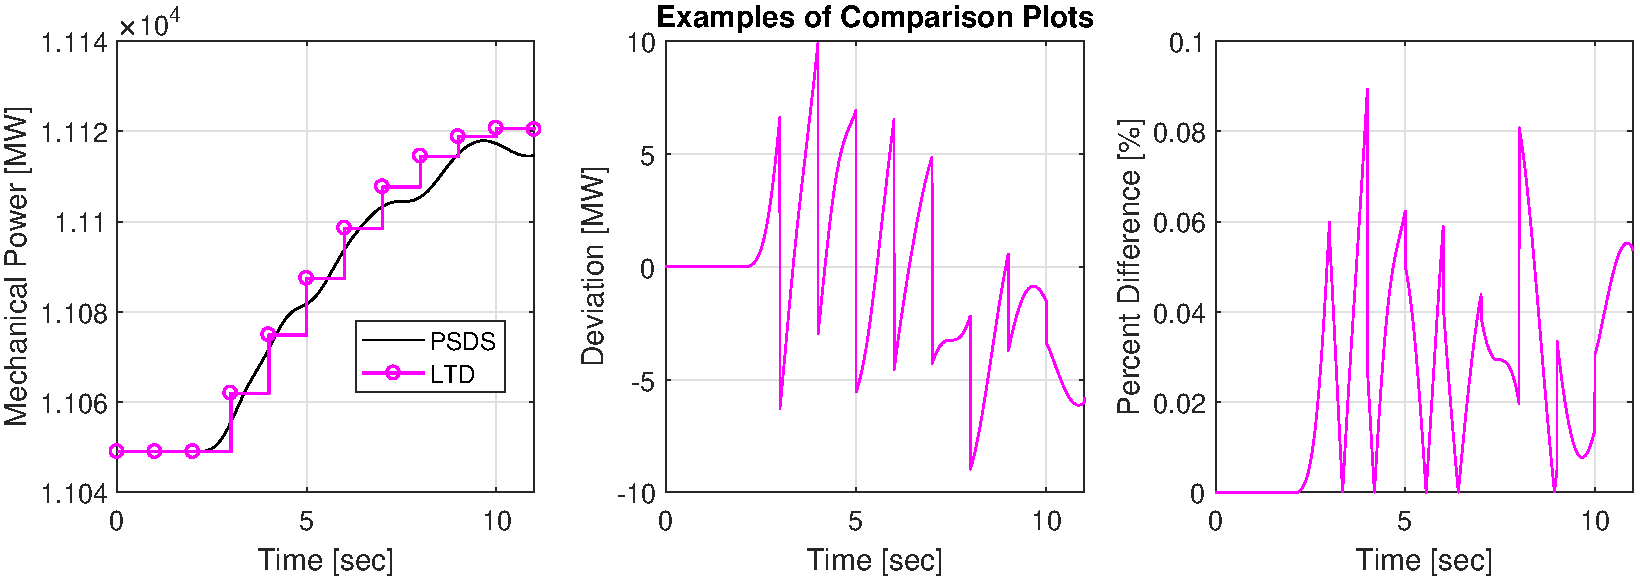
\includegraphics[width=\linewidth]{comparisonsEx} 
		{\footnotesize
		\[\text{PSDS}_{data}-\text{LTD}_{data} = \text{Deviation}_{data}\]
		%Percent difference
		\[\%_{diff} = \dfrac{\abs{x-y}}{\frac{x+y}{2}}*100\% \]}
\end{frame}
%------------------------------------------------



\begin{frame}
\frametitle{Step Perturbance Validation}
\framesubtitle{400 MW Load Step Frequency Comparison}
\begin{columns}
	\begin{column}{.5\linewidth}
		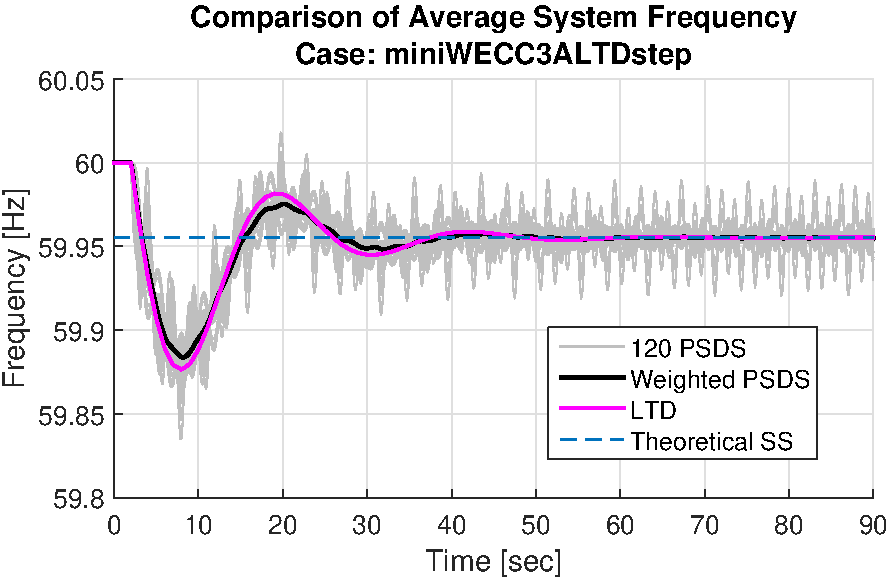
\includegraphics[width=\linewidth]{../../ResearchDocs/TEX/one-offs/final-validation-01/figures/miniWECC3ALTDstepF3}
	\end{column}
	\begin{column}{.5\linewidth}
		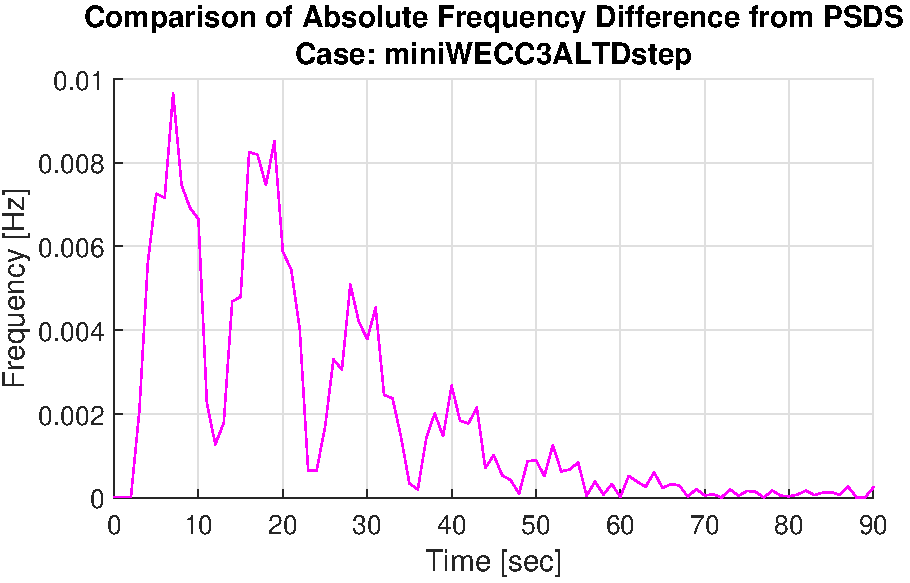
\includegraphics[width=\linewidth]{../../ResearchDocs/TEX/one-offs/final-validation-01/figures/miniWECC3ALTDstepRelF}
	\end{column}
\end{columns}
\end{frame}
%------------------------------------------------
\begin{frame}
\frametitle{Step Perturbance Validation}
\framesubtitle{400 MW Load Step Mechanical Power Comparison}
\begin{columns}
	\begin{column}{.5\linewidth}
		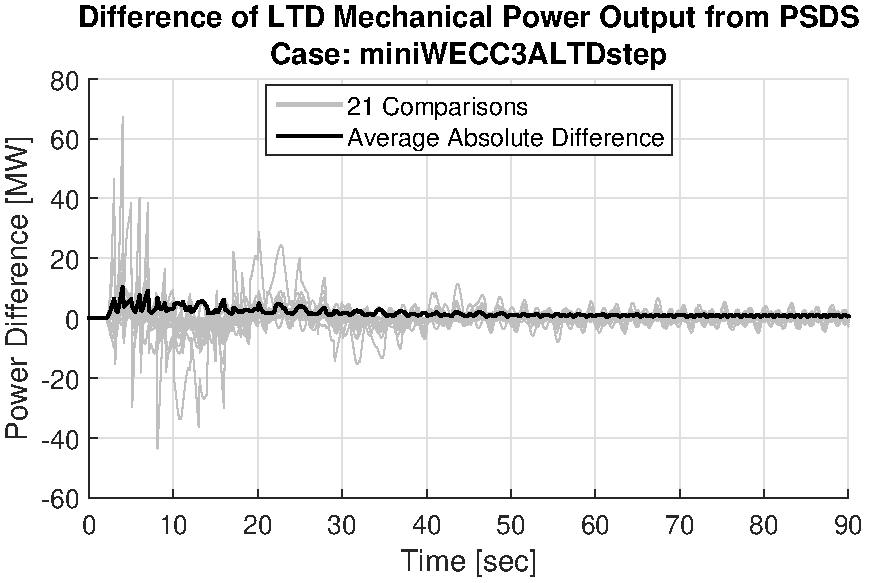
\includegraphics[width=\linewidth]{../../ResearchDocs/TEX/one-offs/final-validation-01/figures/miniWECC3ALTDstepPm2}
	\end{column}
	\begin{column}{.5\linewidth}
		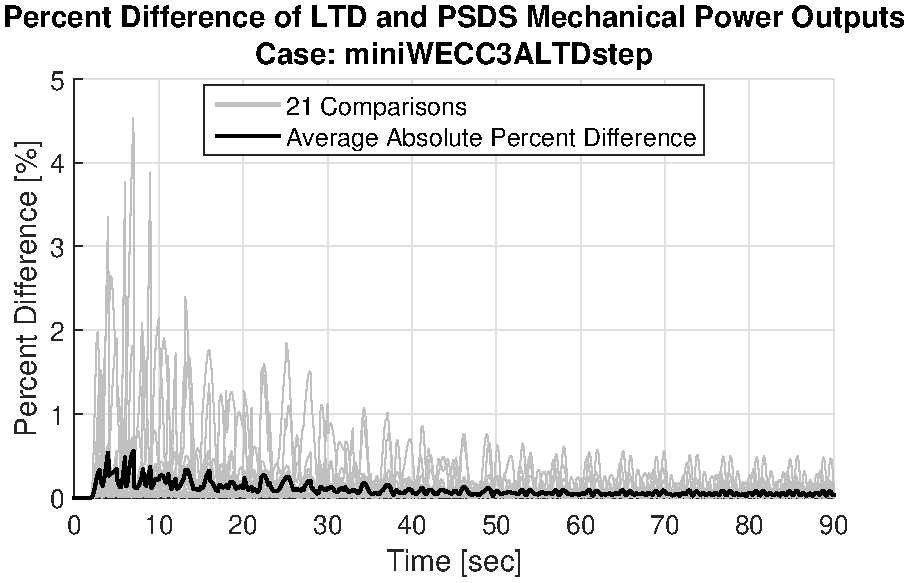
\includegraphics[width=\linewidth]{../../ResearchDocs/TEX/one-offs/final-validation-01/figures/miniWECC3ALTDstepPm3}
	\end{column}
\end{columns}
\end{frame}
%------------------------------------------------
\begin{frame}
\frametitle{Ramp Perturbance Validation}
\framesubtitle{20 second 400 MW Load Ramp Frequency Comparison}
\begin{columns}
	\begin{column}{.5\linewidth}
		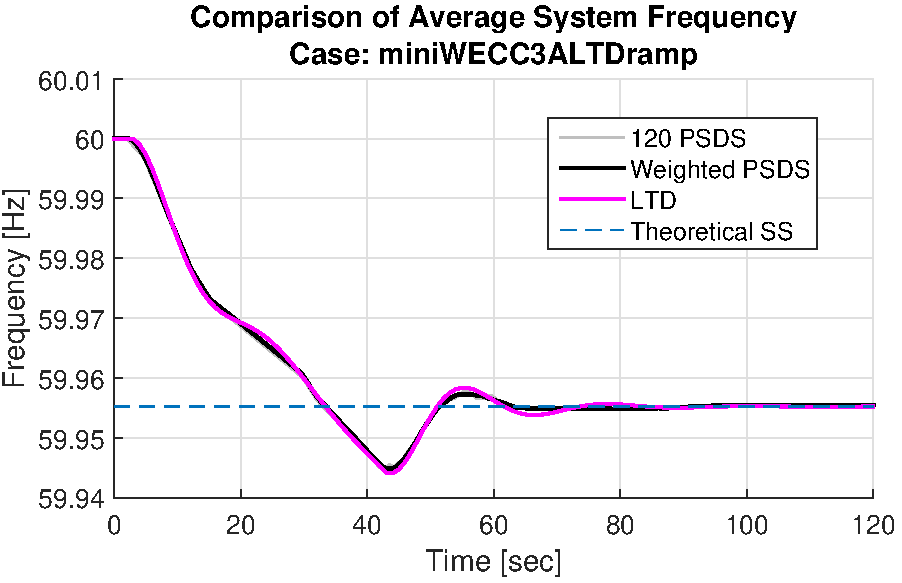
\includegraphics[width=\linewidth]{../../ResearchDocs/TEX/one-offs/final-validation-01/figures/miniWECC3ALTDrampF3}
	\end{column}
	\begin{column}{.5\linewidth}
		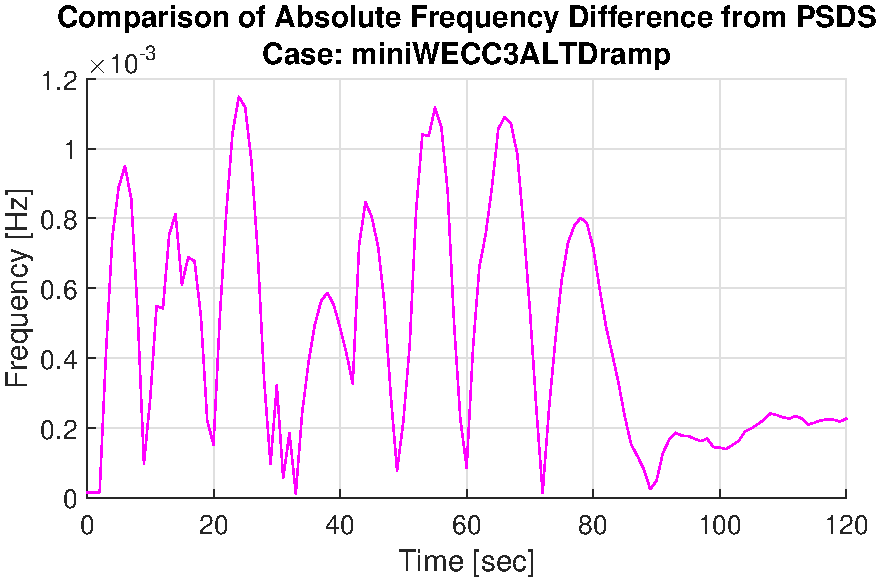
\includegraphics[width=\linewidth]{../../ResearchDocs/TEX/one-offs/final-validation-01/figures/miniWECC3ALTDrampRelF}
	\end{column}
\end{columns}
\end{frame}
%------------------------------------------------
\begin{frame}
\frametitle{Ramp Perturbance Validation}
\framesubtitle{20 second 400 MW Load ramp Mechanical Power Comparison}
\begin{columns}
\begin{column}{.5\linewidth}
	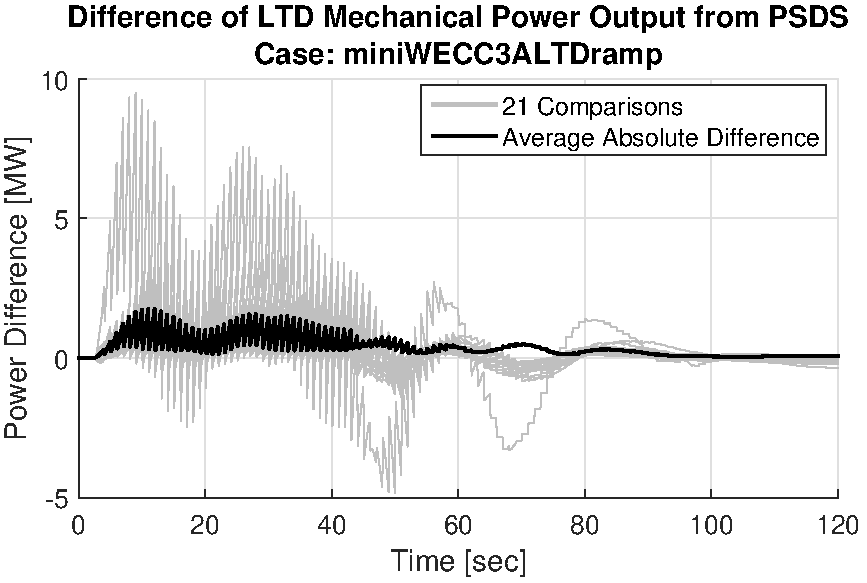
\includegraphics[width=\linewidth]{../../ResearchDocs/TEX/one-offs/final-validation-01/figures/miniWECC3ALTDrampPm2}
\end{column}
\begin{column}{.5\linewidth}
	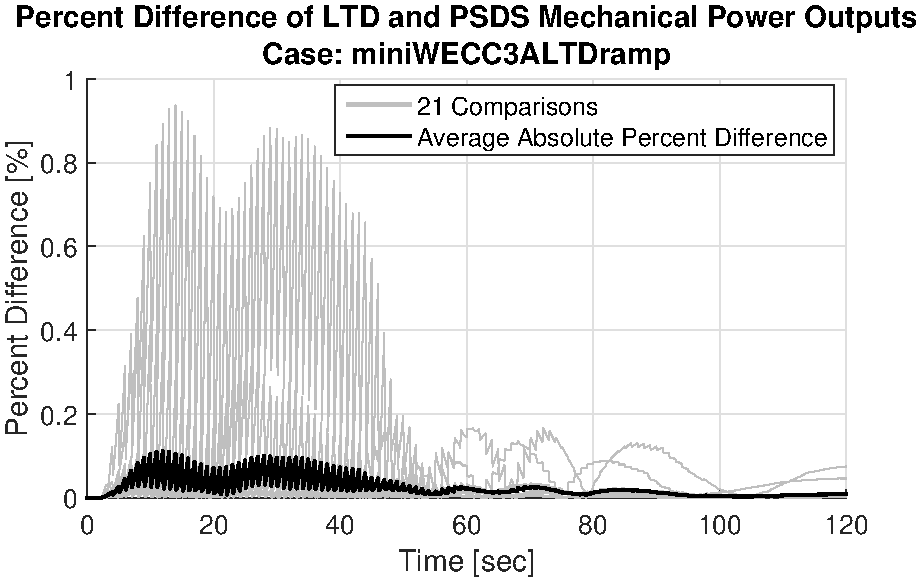
\includegraphics[width=\linewidth]{../../ResearchDocs/TEX/one-offs/final-validation-01/figures/miniWECC3ALTDrampPm3}
\end{column}
\end{columns}
\end{frame}
%------------------------------------------------
\subsection{Quick Controller Test}
%------------------------------------------------
\begin{frame}
\frametitle{Area Droop and Valve Travel}
\begin{columns}
\begin{column}{.5\linewidth}
{\tiny Area 3 droop = 0.2}
	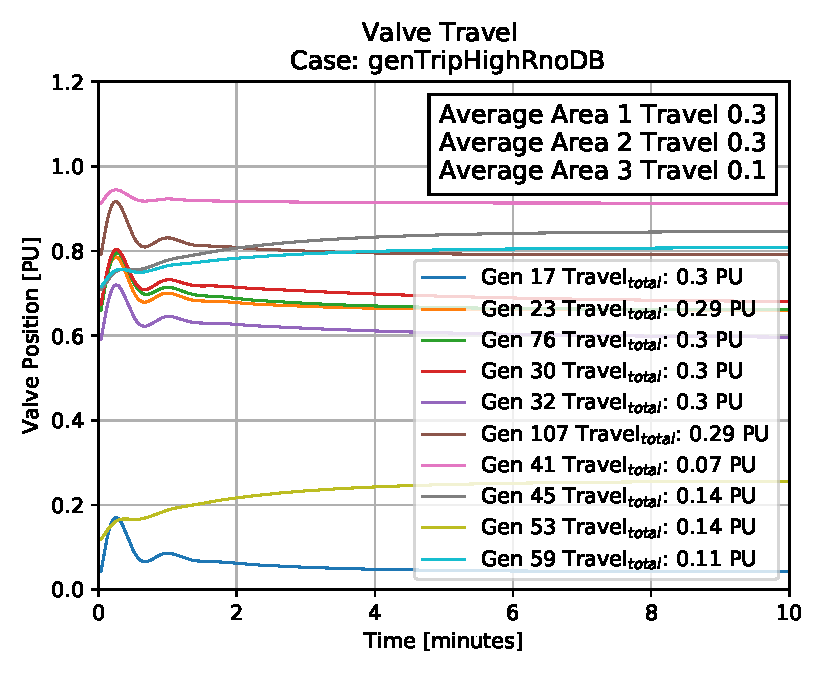
\includegraphics[width=\linewidth]{genTripHighRnoDBValveTravel01}
\end{column}
\begin{column}{.5\linewidth}
{\tiny Area 3 droop = 0.05}
	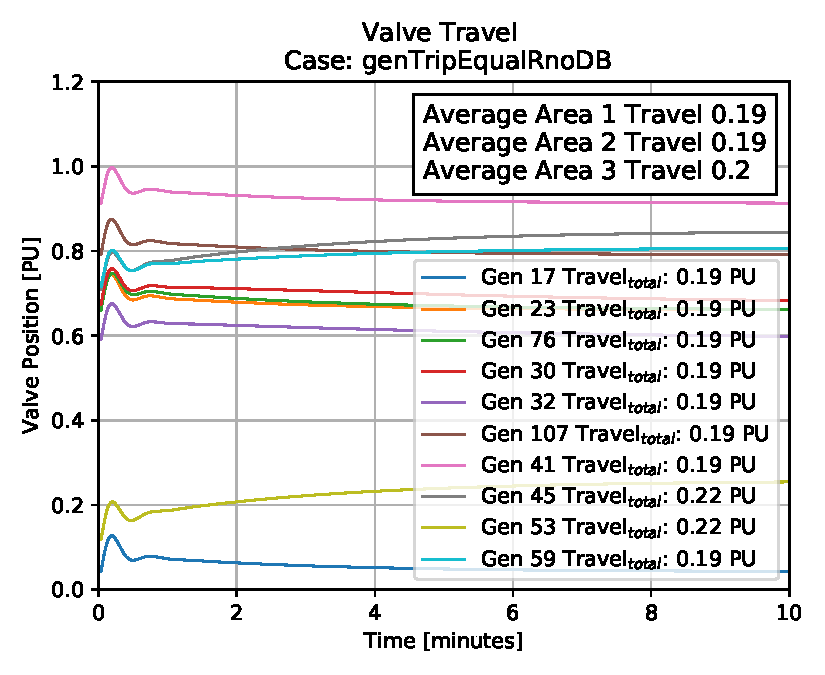
\includegraphics[width=\linewidth]{genTripEqualRnoDBValveTravel01}
\end{column}
\end{columns}
\end{frame}
%------------------------------------------------
\begin{frame}
\frametitle{Deadband and Valve Travel}
\begin{columns}
\begin{column}{.5\linewidth}
{\tiny Step Deadband}
	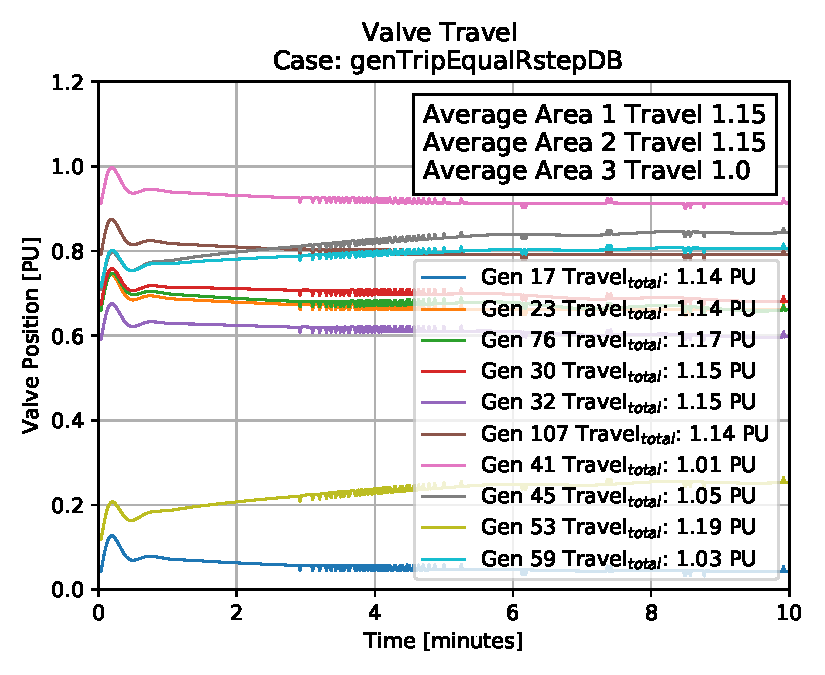
\includegraphics[width=\linewidth]{genTripEqualRstepDBValveTravel01}
\end{column}
\begin{column}{.5\linewidth}
{\tiny Non-Linear Droop Deadband}
	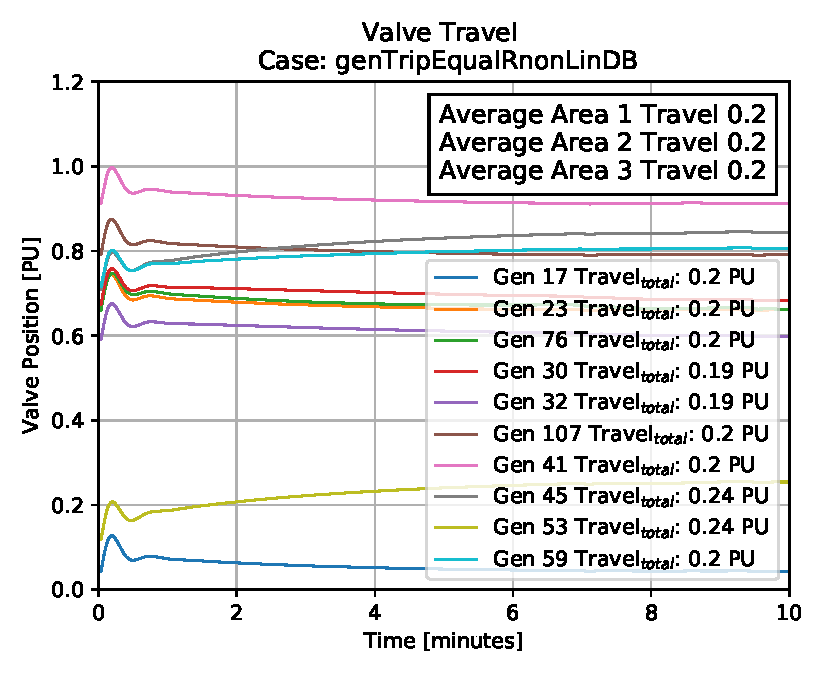
\includegraphics[width=\linewidth]{genTripEqualRnonLinDBValveTravel01}
\end{column}
\end{columns}
\end{frame}
%------------------------------------------------
%************************************************
\section{Final Bits}
%------------------------------------------------
\begin{frame}
\frametitle{Current Conclusions}
\begin{itemize}
	\item Software (PSLTDSim) output appears valid for tested systems.
	\item Governor droop in one area affects how other areas respond.
	\item Step deadband may increase valve travel.
	%\item Governor and AGC interactions can happen easily.
	%\item Advanced control can be used to limit governor and AGC conflicts as well as reduce overall machine effort.
\end{itemize}
\end{frame}
%------------------------------------------------
\begin{frame}
\frametitle{Continuing Work}
\begin{itemize}
\item Experiments with AGC and governor settings.
\item Use of valve travel and system reliability to gauge validity of control regime.
\item Expansion of software capabilities to handle full WECC.
\end{itemize}
\end{frame}
%------------------------------------------------

\begin{frame}
\begin{center}
\Huge{Questions?}
\end{center}
\end{frame}

%-------------------------------------------------
% attempt at having references in slide...
\begin{frame}[allowframebreaks]
\frametitle{References}
\renewcommand*{\bibfont}{\scriptsize} % makes references a resonable size
\printbibliography
\end{frame}



\begin{comment} % Unused slides
%------------------------------------------------
\subsection{Transient Simulation Differences}
%------------------------------------------------
\begin{frame}
\frametitle{Transient vs Long-Term Simulation}
Time scale.
Level of detail required.
Equations - transient simulation uses many ODEs to find next steady state and uses very small timesteps, 
PSLTDSim uses ODE to find next guess of certain inputs to the power flow which then computes the next steady state - uses much large time steps.
\end{frame}

%------------------------------------------------
\begin{frame}
\frametitle{Automatic Generation Control}
%(AGC), also knows as Load Frequency Control or LFC)
%\\
Adjusts generator nominal operating set point to remove any inadvertent interchange and restore system frequency to 60 Hz. Classified Secondary Control.

ACE Conventions Positive ACE denotes over generation. $B$ (the frequency bias) is negative.
\begin{align*}
\text{ACE}_{\text{tie line}} &= P_{\text{interchange}} - P_{\text{sched interchange}}\\
\text{ACE}_{\text{frequency bias}} &= 10B(f_{\text{actual}}-f_{\text{sched}})f_{base}\\
\text{ACE} &= \text{ACE}_{\text{tie line}} -\text{ACE}_{\text{frequency bias}}
\end{align*}
\end{frame}
%------------------------------------------------
\frametitle{And why?}
\begin{itemize}
\item Simplification
\item Facilitate other research
\end{itemize}
\end{frame}
%------------------------------------------------
\begin{frame}
\frametitle{Engineering Areas of Interest}


%------------------------------------------------
\begin{frame}
\frametitle{Project Software Goals}
\begin{itemize}
\item Develop software for (long-term dynamic) LTD simulations.
\item Incorporate useful parts of GE software (PSLF):
\begin{itemize}
	\item Power Systems ($.sav$ files)
	\item Dynamic model data ($.dyd$ files)
	\item Power-flow solver
\end{itemize}
\item Create simplified dynamic models compatible with LTD time steps.
\end{itemize}
\end{frame}

%------------------------------------------------
%************************************************
\section{Background Information}
%________________________________________________

%************************************************
\section{Simulation Model}
%________________________________________________
\subsection{Assumptions, Coding Decisions, Approaches, and Software Operation.}
%------------------------------------------------
\begin{frame}
This simulation assumes:
\begin{enumerate}
\item Time steps of 0.5 to 1 second.
\item Fast dynamics are 'mostly' ignored.
\item System remains synchronized.
\item System frequency is described by the combined PU swing equation:
\setcounter{assumptions}{\value{enumi}} % allow for break in counting
\end{enumerate}
\[ \dot{\omega}_{sys} = \dfrac{1}{2H_{sys} } \left( \dfrac{P_{acc, sys} }{\omega_{sys}(t)} - D_{sys}\Delta\omega_{sys}(t)  \right)\] 
\begin{enumerate}
\setcounter{enumi}{\value{assumptions}}
\item No system damping $(D_{sys} = 0)$.
\end{enumerate}
\end{frame}
%------------------------------------------------

\begin{frame}
Software used:
\begin{itemize}
\item Python 3, IronPython
\item Erlang / AMQP
\item MATLAB
\end{itemize}
\end{frame}
%------------------------------------------------
\begin{frame}
\begin{itemize}
\item Agent\\ An autonomous individual object with properties and methods in a computer simulation.
\item Agent-Based Modeling\\ The idea that a system can be modeled using agents in an environment, and a description of agent-agent and agent-environment interactions. \tiny[2]
\end{itemize}
\end{frame}
%------------------------------------------------
\end{comment}
\end{document}